%%%%%%%%%%%%%%%%%%%%%%%%%%%%%%%%%%%%%%%%%%%%%%%%%%%%%%%%%%%%%%%%%%%%%%%%%%%%%%%%%
%% Version 0.5 // April 2025
%% %%%%%%%%%%%%%%%%%%%%%%%%%%%%%%%%%%%%%%%%%%%%%%%%%
%% Rubén Fernández González
%%  - rferng19@estudiantes.unileon.es
%% %%%%%%%%%%%%%%%%%%%%%%%%%%%%%%%%%%%%%%%%%%%%%%%%%
\documentclass[11pt]{article}
\usepackage{FAP_style}
\usepackage{comment}

\usepackage{multirow}
\usepackage{diagbox}
\usepackage{xfrac}
\usepackage{tikz}
\usepackage{caption, subcaption}
\usepackage{lscape}
\usepackage{pgfplots}
\pgfplotsset{compat=1.18}
\usepackage[export]{adjustbox}
\usepackage{xcolor}

%% ===============================================
%% Setting the line spacing (3 options: only pick one)
% \doublespacing
% \singlespacing
\onehalfspacing
%% ===============================================

\setlength{\droptitle}{-5em} %% Don't touch

% %%%%%%%%%%%%%%%%%%%%%%%%%%%%%%%%%%%%%%%%%%%%%%%%%%%%%%%%%%
% SET THE TITLE
% %%%%%%%%%%%%%%%%%%%%%%%%%%%%%%%%%%%%%%%%%%%%%%%%%%%%%%%%%%
% TITLE:
\title{Sistema Inteligente de Detección, Identificación y Análisis de Vehículos
}

% AUTHORS:
\author{Rubén Fernández González\\
    \href{mailto:rferng19@estudiantes.unileon.es}{\texttt{rferng19@estudiantes.unileon.es}
    }
}    
% DATE:
\date{\today}

% %%%%%%%%%%%%%%%%%%%%%%%%%%%%%%%%%%%%%%%%%%%%%%%%%%%%%%%%%%
% %%%%%%%%%%%%%%%%%%%%%%%%%%%%%%%%%%%%%%%%%%%%%%%%%%%%%%%%%%
\begin{document}
% %%%%%%%%%%%%%%%%%%%%%%%%%%%%%%%%%%%%%%%%%%%%%%%%%%%%%%%%%%
% %%%%%%%%%%%%%%%%%%%%%%%%%%%%%%%%%%%%%%%%%%%%%%%%%%%%%%%%%%
% ABSTRACT
% %%%%%%%%%%%%%%%%%%%%%%%%%%%%%%%%%%%%%%%%%%%%%%%%%%%%%%%%%%
% %%%%%%%%%%%%%%%%%%%%%%%%%%%%%%%%%%%%%%%%%%%%%%%%%%%%%%%%%%
{\setstretch{.8}
\maketitle
% %%%%%%%%%%%%%%%%%%
\begin{abstract}
% Insert the abstract content here--------------------------------------
Esta es una propuesta de investigación sobre el diseño e implementación de una prueba de concepto de un sistema inteligente para la detección, identificación y análisis de vehículos en entornos reales (cámaras embarcadas y puntos fijos como peajes). El sistema integrará técnicas de visión por computador y de aprendizaje profundo para detectar e identificar vehículos en vídeo en tiempo real.
% A paragraph summarizing the content of the Research proposal, including (i) the research line selected, (ii) the problem to be solved, (iii) the selected algorithm/method and (iv) the results obtained from that algorithm/method in different datasets from the literature

% END CONTENT ABS------------------------------------------
\noindent
\textit{\textbf{Keywords: } Detección de vehículos, Identificación, Deep Learning, Cámaras embarcadas} \\ %% <-- Keywords HERE!
\noindent

\end{abstract}
}





% %%%%%%%%%%%%%%%%%%%%%%%%%%%%%%%%%%%%%%%%%%%%%%%%%%%%%%%%%%
% %%%%%%%%%%%%%%%%%%%%%%%%%%%%%%%%%%%%%%%%%%%%%%%%%%%%%%%%%%
% BODY OF THE DOCUMENT
% %%%%%%%%%%%%%%%%%%%%%%%%%%%%%%%%%%%%%%%%%%%%%%%%%%%%%%%%%%
% %%%%%%%%%%%%%%%%%%%%%%%%%%%%%%%%%%%%%%%%%%%%%%%%%%%%%%%%%%

% --------------------
\section{Introducción}
% --------------------

La detección e identificación de vehículos en tiempo real es una tarea muy importante actualmente, debido al crecimiento de la industria de coches autónomos (y otros también no autónomos), donde unos sensores se encargan de detectar otros vehículos en las proximidades para poder razonar y actuar gracias a esta información, como pueden ser unos sensores en distintas partes del vehículo para que, al aparcar, puedan detectar y medir distancias a un vehículo próximo. Y no solo es importante para los coches autónomos también lo es para:
\begin{itemize}
    \item \textbf{Control del tráfico:} Por ejemplo, se puede implementar un programa para que detecte y cuente la cantidad y tipo de vehículos de una intersección para variar dinámicamente el estado de los semáforos.
    \item \textbf{Coches robados:} Simplemente se puede hacer una detección de los coches y compararlos uno a uno con una base de datos de coches, o vehículos en general, robados y poder realizar avisos a la policía.
\end{itemize}

La detección y reconocimiento precisa de un vehículo no es una tarea sencilla, incluso para los humanos diferenciar entre muchas marcas existentes y aún más, entre los diferentes modelos de cada una de las marcas, es una tarea sumamente compleja. Las redes neuronales permiten hacer esta tarea de forma eficaz y precisa, pudiéndose comunicar con otro tipo de programas de señales o emergencias, por ejemplo.

En general, la mayoría de investigadores usan alguno de los tantos modelos YOLO existentes. Ya que YOLO destaca en cualquier tipo de tarea gracias a su flexibilidad, es especialmente prominente a dar buenos resultados en la tarea de detección y reconocimiento de vehículos. Un ejemplo claro puede ser el caso del proyecto de \textbf{Sarvesh Shirulkar} et Al. \cite{ramzan2023enhancingvehicleentranceparking} con YOLO para controlar las señales de tráfico según las detecciones del modelo YOLO. Otro ejemplo es el de \textbf{Anning Ji y Xintao Ma} \cite{JI2025804}, en el que utilizan como base un modelo YOLO10 al que se le modifica la parte de extracción de características. Aunque estos modelos predominen la elección de investigadores, hay otras opciones con diferentes arquitecturas que pueden ser muy útiles en determinados escenarios, como puede ser la red neuronal de \textbf{Leyre Encio} et Al. \cite{articleEncio} basada en CenterNet, que trata de asimilar un diseño similar a la de los transformadores con su \textit{encoder-decoder}.

En la sección \ref{sec:literatureReview} o \textbf{Estado del arte}, se nombran varios métodos, principalmente con modelos YOLO, para detectar y reconocer todo tipo de vehículos en distintos entornos. Los modelos (o métodos) seleccionados se explicarán detalladamente en la sección \ref{sec:selectedMethod} o \textbf{Métodos seleccionados}. En la sección \ref{sec:datasets} o \textbf{Datasets} se disponen los conjuntos de datos de vehículos que se van a utilizar para entrenar y probar los modelos. 





% --------------------
\section{Estado del arte}
% --------------------
% Insert the content of the proposed solutions here. Text from the guide is inserted as a reference for you to be aware of where the text could be inserted in LaTeX.
\label{sec:literatureReview}

K. Saiveena y P. Praaven \cite{SAIVEENA2026111086} tienen un enfoque de detección y segmentación de vehículos basado en \textit{Edge Intelligence} (EI), una rama de \textit{Deep Learning}. El programa, \textbf{ViT-YOLOv5}, se divide en dos partes fundamentales: la primera es un ViT \textit{(Vision Transformer)}, encargado de \textbf{extraer y procesar las características} de las imágenes sustituyendo la labor del extractor de características del detector \textbf{YOLOv5} \footnote{Accesible a través de GitHub: \url{https://github.com/ultralytics/yolov5}}: \textbf{CSPDarknet}. Esta integración permite capturar de manera más eficiente tanto las características globales como las locales. La segunda parte consta del detector \textbf{YOLOv5}, que se encarga de generar las predicciones de clase, su confianza y las \textit{bounding boxes}. Para medir el rendimiento de este proyecto se obtuvieron 4 datasets de vehículos (dirigidos a detección de objetos principalmente) de la web de Kaggle \footnote{Accesibles a través de: \href{https://www.kaggle.com/datasets/sakshamjn/vehicle-detection-8-classes-object-detection}{Sakshamjn}, \href{https://www.kaggle.com/datasets/saumyapatel/traffic-vehicles-object-detection}{Saumyapatel}, \href{https://www.kaggle.com/datasets/seyeon040768/car-detection-dataset}{Seyeon} y \href{https://www.kaggle.com/datasets/nadinpethiyagoda/vehicle-dataset-for-yolo}{Nadinpethiyagoda}}, alcanzando un \textit{accuracy} de \textbf{97.25\%}, \textbf{94.42\%}, \textbf{94\%} y \textbf{95.7\%} para cada dataset, respectivamente. Un análisis profundo con diferentes configuraciones y modelos se puede observar en la figura \ref{fig:vit-yolo}, con diferencias notables entre el \textbf{YOLOv5} base y el modificado con el transformador, \textbf{ViT-YOLOv5}. Este modelo se ha entrenado en una NVIDIA Tesla V100 GPU de 32GB de RAM.

\begin{figure}[htb]
\centering
    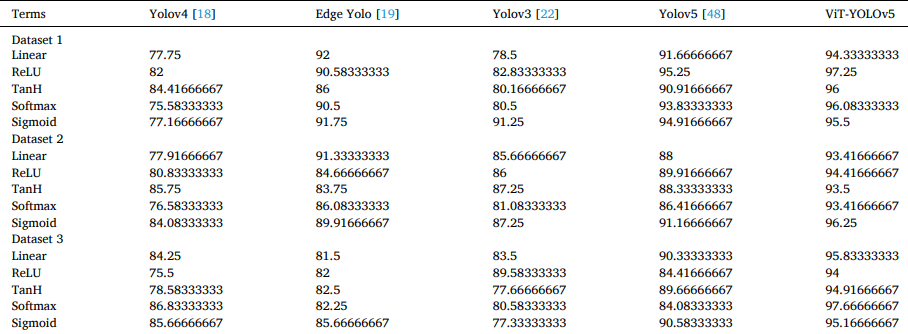
\includegraphics[width=.85\textwidth]{figures/vit-yolo.png}
    \caption{Rendimiento de diferentes modelos y configuraciones en los datasets de vehículos\\
    \footnotesize{Fuente: \textit{https://www.sciencedirect.com/science/article/pii/S0045790626001588}}}
    \label{fig:vit-yolo}
\end{figure}



La identificación precisa de objetos en la gestión del tráfico urbano y el transporte autónomo es clave y, por eso, Wenjie Zhu et Al. \cite{ZHU2026120336} proponen el modelo \textbf{DFEM-Net} \footnote{El modelo es completamente accesible a través de \url{https://github.com/ahtarv/DFEM-Net}} que \textbf{mejora la flexibilidad} al aprender diversas formas, tamaños y detalles superficiales, algo que es muy importante a la hora de realizar este tipo de tareas. El primer cambio es el \textbf{ajuste dinámico del tamaño} y de la forma de los kernels convolucionales a través de una \textbf{TuaNet}: una integración de una \textbf{DCN} \textit{(Deformable Convolutional Network)} junto con \textbf{Tua Attention}. Además, se introduce un módulo de fusión de características multi-escala \textbf{Scalseq}, que ayuda a la red a \textbf{extraer características a distintos niveles}. Al mismo tiempo, un módulo \textbf{Zoomcat} de triple cifrado de características \textbf{reduce el solapamiento} para superponer pequeños objetos. Este método obtiene un \textbf{77.5\%} de mAP@0.5 y un \textbf{59.3\%} de mAP@0.5:0.95 en el \textbf{TVAP-Normal Dataset}, y un \textbf{71.3\%} de mAP@0.5 y un \textbf{46.5\%} de mAP@0.5:0.95 en el \textbf{TVAP-Foggy Dataset}. En comparación, YOLOv8 obtiene un 74.6\% de mAP@0.5 y un 57.6\% de mAP@0.5:0.95 en el TVAP-Normal dataset, algo que se puede observar con 4 imágenes del dataset en la figura \ref{fig:tvap}. El entrenamiento se ha realizado durante 400 iteraciones con un optimizador SGD y una tasa de aprendizaje inicial de 0.01 con un decaimiento de 0.0005 en una Tesla V100-SXM2-16GB GPU. Además, \textbf{DFEM-Net} mantiene una alta eficiencia computacional con \textbf{9.1 GFLOPs}, comparable con los 8.7 GFLOPs de la versión más pequeña de YOLOv8.

\begin{figure}[htb]
\centering
    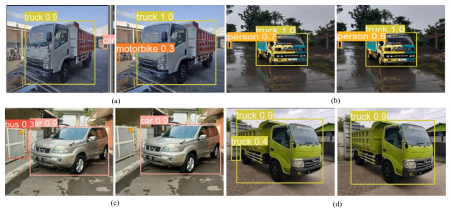
\includegraphics[width=.85\textwidth]{figures/tvap_example.png}
    \caption{Resultados de YOLOv8 (izquierda) y DFEM-Net (derecha) en 4 distintas imágenes del dataset TVAP-Normal\\
    \footnotesize{Fuente: \textit{https://www.sciencedirect.com/science/article/pii/S026322412600045X}}}
    \label{fig:tvap}
\end{figure}



Un framework unificado y optimizado de detección, tracking, conteo, predicción de movimiento y clasificación de vehículos es presentado por Mohammed Alnusayri et Al. \cite{ALNUSAYRI2026}. El framework consta de \textbf{YOLOv10}, \textbf{ByteTrack}, \textbf{Optical-flow density estimation}, predicción de trayectorias con \textbf{Long Short-Term Memory-based (LSTM-based)} y extracción de características con \textbf{Speeded-Up Robust Feature (SURF)} y \textbf{Gray-Level Co-occurrence Matrix (GLCM)} junto al modelo \textbf{VGG16}. Los conjuntos de datos utilizados son \textbf{UAVid} y \textbf{UAVdt}\footnote{Los datasets son accesibles por \href{https://research.utwente.nl/en/datasets/uavid-dataset/}{UAVID} y \href{https://sites.google.com/view/daweidu/projects/uavdt}{UAVDT}}, cuyas imágenes están a una altura de unos 50-70 metros de altura, en los que el framework alcanza una precisión en la detección de \textbf{95.49\%}, \textbf{95.15\%} en recall y \textbf{95.52\%} en f1-score. Algunos ejemplos se pueden ver sobre la figura \ref{fig:art3}. Las pruebas se han realizado sobre una Intel i7-12700K (3.6 GHz), 32 GB RAM y una NVIDIA RTX 3090 GPU.

\begin{figure}[htb]
\centering
    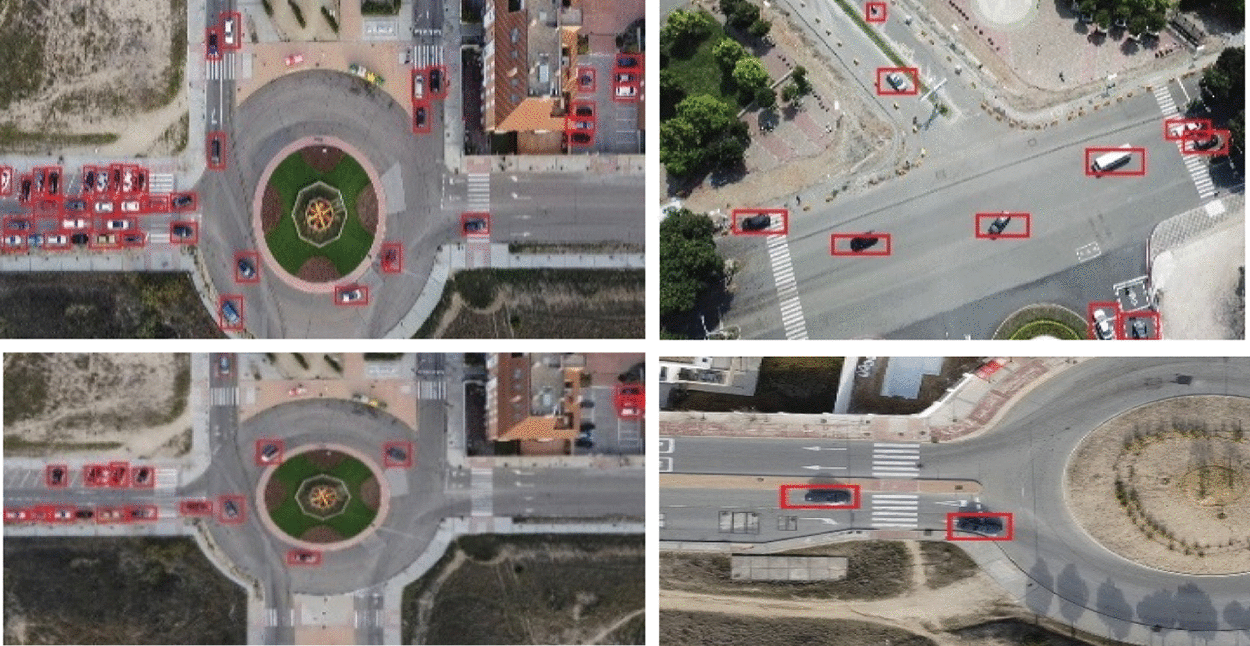
\includegraphics[width=.85\textwidth]{figures/art3.png}
    \caption{Ejemplo de detección de vehículos sobre una vista UAV\\
    \footnotesize{Fuente: \textit{https://www.sciencedirect.com/org/science/article/pii/S1546221826000974}}}
    \label{fig:art3}
\end{figure}



La detección de objetos pequeños y condiciones de tráfico son un desafío para la gestión del tráfico, así que Anning Ji y Xintao Ma \cite{JI2025804} desarrollan un framework de detección muy novedoso: \textbf{YDFNet}, que integra \textbf{YOLOv10} para extraer rápidamente las características, una \textbf{BiFPN} \textit{(Bidirectional Feature Pyramid Network)}, cuya arquitectura se puede observar en la figura \ref{fig:bifpn}, para fusionar las características a distintas escalas y un transformador de detección \textbf{DETR}. Este framework utiliza las ventajas de cada una de las partes para mejorar la eficiencia y precisión de la detección. Para experimentar, se escogen los datasets \textbf{UA-DETRAC} y COCO\footnote{Los datasets son obtenibles por \href{https://www.kaggle.com/datasets/bratjay/ua-detrac-orig}{UA-DETRAC} y \href{https://cocodataset.org}{COCO}}, en los que alcanza un \textbf{75.8\%} de mAP y un \textbf{52.2\%} de AP\textsubscript{small} mejorando resultados anteriores como los de YOLOv10 en los mismos datasets: 67.8\% de mAP y un 42.5\% de AP\textsubscript{small}. Las pruebas fueron realizadas en entornos con restricciones de recursos a través de NVIDIA Jetson AGX Xavier and Rockchip RK3588.

\begin{figure}[htb]
\centering
    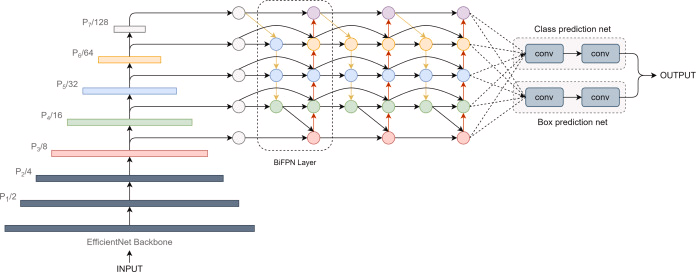
\includegraphics[width=.85\textwidth]{figures/bifpn.png}
    \caption{Arquitectura de una FPN bidireccional (BiFPN)\\
    \footnotesize{Fuente: \textit{https://www.sciencedirect.com/science/article/pii/S1110016825007999}}}
    \label{fig:bifpn}
\end{figure}



Otro avance necesario en la gestión del tráfico es el de anomalías, Seyed H.H.D. et Al. \cite{dolatabadi2025revolutionizingtrafficmanagementaipowered} proponen un sistema en tiempo real de detección de vehículos, anomalías de tráfico y comportamiento de los conductores. El sistema integra datos geoespaciales y del tiempo para adaptarse a condiciones cambiantes. Los modelos utilizados son \textbf{YOLOv8} y \textbf{YOLOv11}. Las imágenes fueron adquiridas a través de varios datasets de imágenes de tráfico en determinadas áreas de tráfico de la provincia de Isfahan, Irán. Además, las imágenes fueron adquiridas desde distintos ángulos para replicar las perspectivas de las cámaras de vigilancia. Los resultados obtenidos para cada uno de los modelos, en cuestión de tanto detección de vehículos como de anomalías, se pueden observar en la tabla \ref{tab:v8-11}.

\begin{table}[htb]
    \centering
    \begin{tabular}{|c|c|c|c|c|}
         \hline   
         \textbf{Modelo} & \textbf{Precision} & \textbf{Recall} & \textbf{mAP50} & \textbf{mAP50-95}\\
         \hline
         \textbf{YOLOv8} & 86.1\% & 73.0\% & 87.4\% & 68.2\%\\ 
         \hline
         \textbf{YOLOv11} & 89.7\% & 72.3\% & 81.3\% & 62.4\%\\
         \hline
    \end{tabular}
    \caption{Resultados de YOLOv8 y YOLOv11 en entornos de tráfico}
    \label{tab:v8-11}
\end{table}



En cámaras de monitorización estáticas, las imágenes son tomadas automáticamente: sin tener la garantía de que los objetos de interés (en este caso los vehículos) se puedan apreciar con claridad, ya sea por clima, la localización de la cámara o que el objeto es parcialmente observable. Para resolver este problema, Sara Beery et Al. \cite{beery2020contextrcnnlongterm} deciden crear una CNN con un módulo de atención de forma que se aprovecha el contexto temporal de los frames no etiquetados para mejorar la precisión, \textbf{Context R-CNN}. En este modelo, donde la base es una \textbf{Faster R-CNN}, las bounding boxes candidatas de la primera parte primero se pasan a través de 2 módulos de atención que indexan en dos depósitos de memoria para \textbf{proveer contexto local y global}. Estos módulos devuelven un vector de características que se pasa a la segunda parte del modelo \textbf{Faster R-CNN} de forma normal. En la figura \ref{fig:context-rcnn} se puede ver el modelo completo. Esta propuesta alcanza un \textbf{42.6\%} de mAP en el dataset CityCam\footnote{El dataset es accesible por \url{https://web.tecnico.ulisboa.pt/~ist12390/public_html/citycam/}}.

\begin{figure}[htb]
\centering
    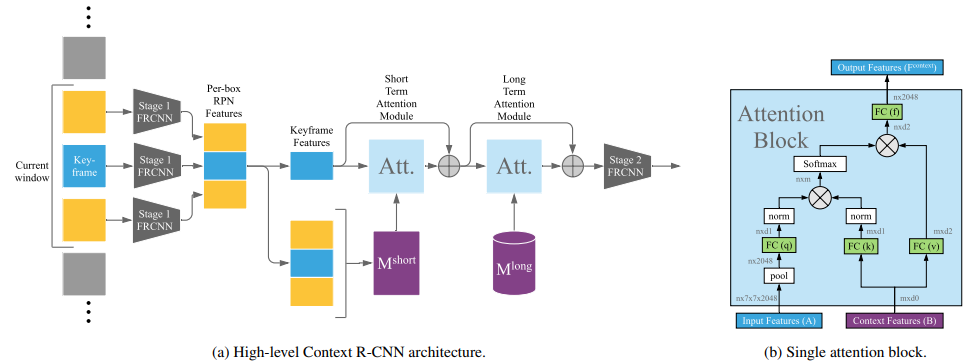
\includegraphics[width=.85\textwidth]{figures/context_rcnn.png}
    \caption{Arquitectura de una Context R-CNN\\
    \footnotesize{Fuente: \textit{https://arxiv.org/pdf/1912.03538}}}
    \label{fig:context-rcnn}
\end{figure}



La gestión automática de la entrada y salida de vehículos en aparcamientos es un desafío en temas de eficiencia y seguridad. Para solucionar esto, Muhammad U.R. et Al. \cite{ramzan2023enhancingvehicleentranceparking} utilizan modelos de vanguardia para la detección del vehículo, verificación de la matrícula, y detección y reconocimiento del conductor; el esquema se puede observar en la figura \ref{fig:doble-yolo}. Después de probar varios modelos, el que más destaca en cada uno de los anteriores apartados es \textbf{YOLOv8n}, la versión más pequeña de \textbf{YOlOv8}, destacando por encima de \textbf{YOLOv5} y \textbf{Faster R-CNN}. Ya que se utilizan 2 modelos para las dos primeras tareas de detección (vehículo y matrícula por separado), se necesitan conjuntos de datos diferentes: para vehículos se recogieron 6000 imágenes de 3 categorías diferentes y para las matrículas se recogen otras 600 de matrículas de coches y bípedos. Para el reconocimiento de rostros se usa \textit{Haar cascades}. El sistema alcanza un \textbf{99.2\%} de precisión, \textbf{99\%} de recall, \textbf{99.4\%} de mAP@50 y \textbf{99.1\%} de IoU, y \textbf{99.1\%} de precisión, \textbf{99.1\%} de recall, \textbf{99.2\%} de mAP@50 y \textbf{98.2\%} de IoU en las tareas de detección de vehículos y detección de matrículas, respectivamente.

\begin{figure}[htb]
\centering
    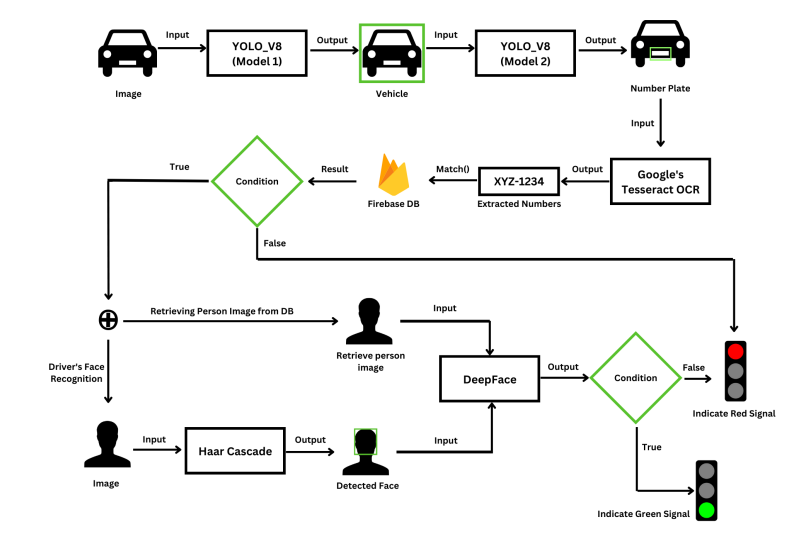
\includegraphics[width=.85\textwidth]{figures/doble_yolo.png}
    \caption{Esquema de flujo de la tarea de detección de vehículos y de matrículas\\
    \footnotesize{Fuente: \textit{https://arxiv.org/pdf/2312.02699}}}
    \label{fig:doble-yolo}
\end{figure}



La congestión del tráfico es un grave problema para países superpoblados, sobre todo ciudades, como en la India. Sarvesh Shirulkar et Al. \cite{10984828} idean un sistema adaptativo para controlar las señales de tráfico en intersecciones usando detección y seguimiento de vehículos en tiempo real con el algoritmo \textbf{YOLO}, reduciendo de gran manera la congestión del tráfico y mejorando la circulación urbana. El funcionamiento de este sistema consta de 5 pasos fundamentales:
\begin{itemize}
    \item Primero se captura la imagen inicial de la cámara de tráfico.
    \item Con YOLO se cuentan los vehículos de cada tipo: camiones, autobuses, coches y motocicletas no tienen el mismo tamaño.
    \item Se calcula la densidad del tráfico, teniendo en cuenta un peso asignado a cada categoría y su influencia en la circulación.
    \item Se modifica dinámicamente el estado y la temporización de la señal verde del semáforo. El resultado se puede observar en la figura \ref{fig:pcu}.
\end{itemize}

\begin{figure}[htb]
\centering
    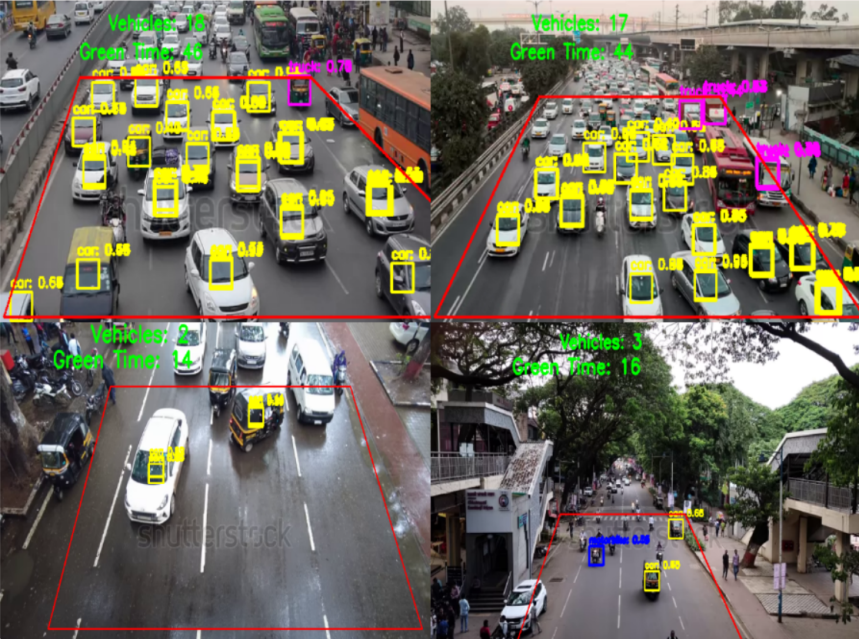
\includegraphics[width=.85\textwidth]{figures/pcu.png}
    \caption{Resultado del sistema con el conteo de vehículos y el temporizador del semáforo\\
    \footnotesize{Fuente: \textit{https://ieeexplore.ieee.org/stamp/stamp.jsp?tp=\&arnumber=10984828}}}
    \label{fig:pcu}
\end{figure}



Este siguiente proyecto de B. Shyamala Gowri et Al. \cite{10988348} desarrolla un sistema de gestión del tráfico que integra la versión \textbf{YOLOv8} para la detección de vehículos y una priorización de las señales de tráfico con \textbf{GNNs (Graph Neural Networks)} para solucionar los problemas de los sistemas de tráfico tradicionales. Estos sistemas fallan a la hora de detectar los vehículos de emergencia y adaptar las señales de tráfico según convenga para ayudar a la circulación. El sistema propuesto junta las capacidades de detección de \textbf{YOLO} con el aprendizaje reforzado de las \textbf{GNNs} para ajustar dinámicamente las señales de tráfico en tiempo real según las condiciones de la carretera. Para el conjunto de datos, se obtuvieron grabaciones de tráfico de cámaras de coches (dashcams), UAVs y cámaras de vigilancia. La detección alcanzó un \textbf{94.7\%} de precision, \textbf{93.5\%} de recall, \textbf{94.1\%} de f1-score y \textbf{9.6 ms} de tiempo de detección en el conjunto de pruebas, una mejora considerable como se puede ver en la figura \ref{fig:yolo8-vdet} comparándolo con otros métodos como \textbf{YOLOv5} y \textbf{Faster R-CNN}. 

\begin{figure}[htb]
\centering
    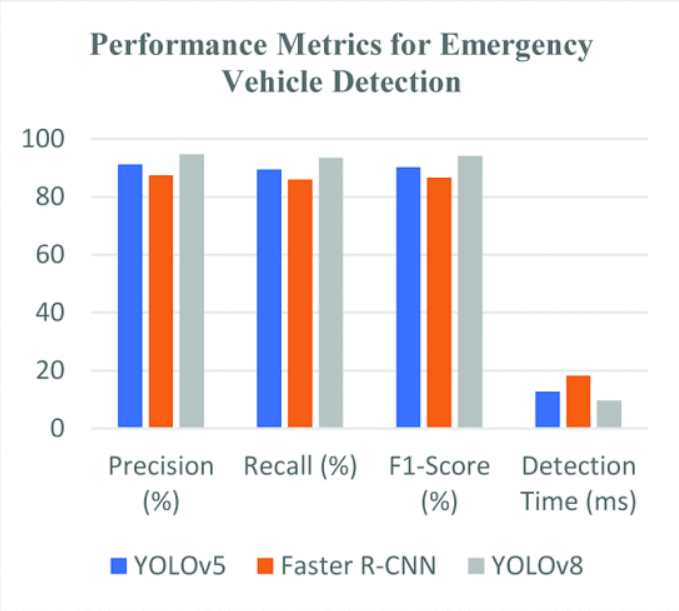
\includegraphics[width=.65\textwidth]{figures/yolo8_vdet.png}
    \caption{Rendimiento de YOLOv8 frente a otros detectores en detección de vehículos\\
    \footnotesize{Fuente: \textit{https://ieeexplore.ieee.org/document/10988348}}}
    \label{fig:yolo8-vdet}
\end{figure}



Otro país con gran densidad en las ciudades es China, donde cada vez los atascos son mas prolíficos a suceder, afectando la vida de las personas y su eficiencia en el trabajo. Para solucionar esto, Xiaohui Guan y Xinxin Sun \cite{9858960} presentan un método de detección de vehículos y estadísticas de tráfico apropiado para cualquier tipo de intersecciones y cruces. Para poder tener un buen modelo entrenado, se extraen únicamente 4 categorías (coches, autobuses, motocicletas y camiones) del dataset \textbf{COCO2017} y todas las imágenes se normalizan a una dimensión de 299 x 299 píxeles. En el entrenamiento con validación cruzada se usa el modelo de detección \textbf{YOLOv3}, con una tasa de aprendizaje de \textbf{1e-4}. Además de probar el modelo de detección con un vídeo, se utiliza el modelo de seguimiento \textbf{DeepSort} para predecir la localización de los vehículos en el siguiente fotograma. Por último, se contabiliza el flujo del tráfico. En el vídeo de pruebas, la intersección se divide en 5 áreas según la figura \ref{fig:intersec}, consiguiendo que el modelo \textbf{YOLO} detecte 472 vehículos en total, donde sólo 9 de ellos se contaron erróneamente.

\begin{figure}[htb]
\centering
    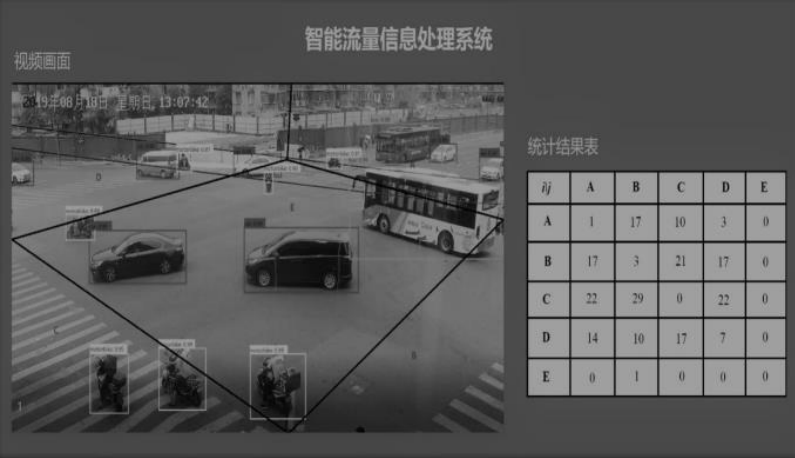
\includegraphics[width=.85\textwidth]{figures/intersec.png}
    \caption{Sistema de detección de vehículos con intersecciones\\
    \footnotesize{Fuente: \textit{https://ieeexplore.ieee.org/document/9858960}}}
    \label{fig:intersec}
\end{figure}



Para solucionar los problemas de detección de vehículos en entornos complejos, Chenyu Gu et Al. \cite{10828068} investigan y diseñan un proyecto para atajar este problema. El primer paso es construir un dataset que incluya entornos complejos e imágenes con vehículos pequeños. El modelo seleccionado es \textbf{YOLOv7}, o al menos la base, ya que integra un canal multiescala y un mecanismo de atención especial: \textbf{Coordinate Attention (CA)}. La estructura completa de este algoritmo modificado, \textbf{YOLOv7-veh}, se muestra en la figura \ref{fig:yolov7-veh}, donde el mecanismo \textbf{CA} funciona como una unidad computacional para \textbf{mejorar la representación de características},  recibiendo características de capas intermedias y mejorando esas mismas características sin cambiar la dimensión. Para la experimentación se utilizó el dataset \textbf{BIT-Vehicle}\footnote{El dataset es accesible por \href{https://www.kaggle.com/datasets/kuanghangdong/bitvehicle}{Bitvehicle}}, el cual contiene 9850 imágenes de vehículos capturadas en diferentes tiempos y escenarios. Debido a las limitaciones de hardware, se construyó un conjunto más pequeño de 4800 imágenes (proporción de entrenamiento/pruebas de 7:3), alcanzando un \textbf{96.2\%} de mAP@0.5 y \textbf{18.9 FPS}, mejorando los 21.7 FPS y 93.5\% de mAP@0.5 del YOLOV7 sin modificar. Las pruebas se han realizado sobre una Intel i9-13900HX CPU de 32 núcleos y una NVIDIA RTX 4090 GPU (12GB de VRAM).

\begin{figure}[htb]
\centering
    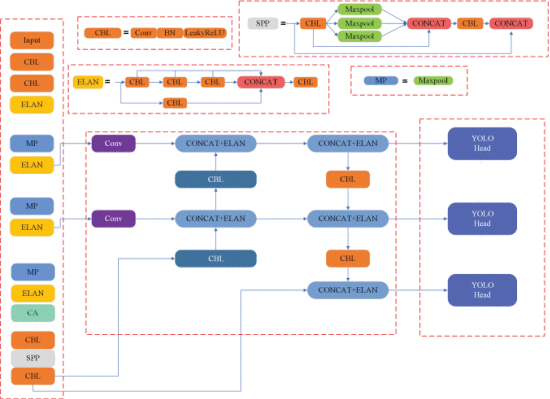
\includegraphics[width=.85\textwidth]{figures/yolov7_veh.png}
    \caption{Arquitectura de YOLOv7-veh\\
    \footnotesize{Fuente: \textit{https://ieeexplore.ieee.org/document/10828068}}}
    \label{fig:yolov7-veh}
\end{figure}



Los vehículos aéreos no tripulados (UAVs) son muy útiles en la tarea de monitorización del tráfico, todo gracias a su capacidad de grabar grandes superficies sin reducir la velocidad del vehículo. En este estudio, Vaishnavee V. R. et Al. \cite{11213146} presentan un proyecto de detección y clasificación de vehículos durante condiciones variadas de luz en entornos de tráfico de la India. El conjunto de datos seleccionado para el entrenamiento y las pruebas, es el dataset \textbf{SHIVNATRAJ}\footnote{El dataset es accesible por \url{https://www.shivnatraj.com}}, que incluye un espectro muy variado de vehículos comunes en carreteras Indias, agrupando categorías como coches, autobuses, motocicletas, camiones, calesas y LCVs. Se seleccionaron 5 modelos para comparar el rendimiento en términos de detección y velocidad: \textbf{YOLOv7}, \textbf{YOLOv8}, \textbf{Faster R-CNN} y el transformador \textbf{DINO-DETR}. Los resultados obtenidos, observables en la tabla \ref{tab:shivnatraj}, muestran que el modelo seleccionado, \textbf{YOLOv8} consigue el mejor balance entre precisión y velocidad. \textbf{YOLOv7} es inferior en precisión, \textbf{DINO-DETR} sufre de una muy baja velocidad de inferencia (8 FPS) y tanto \textbf{YOLOv11} como \textbf{Faster R-CNN} son modelos muy precisos, pero computacionalmente menos óptimos.

\begin{table}[htb]
    \centering
    \begin{tabular}{|c|c|c|c|}
         \hline   
         \textbf{Modelo} & \textbf{FPS} & \textbf{mAP50 (día)} & \textbf{Fortalezas} \\
         \hline
         \textbf{YOLOv7} & 20 FPS & 79\% & Preciso, menos eficiente\\ 
         \hline
         \textbf{YOLOv8} & 15-18 FPS & 81\% & Rápido, ligero\\
         \hline
         \textbf{YOLOv11} & 12 FPS & 83\% & Muy preciso, gran latencia\\
         \hline
         \textbf{Faster R-CNN} & 10 FPS & 80\% & Preciso, gran latencia\\
         \hline
         \textbf{DINO-DETR} & 8 FPS & 84\% & Mejor detección de noche\\
         \hline
    \end{tabular}
    \caption{Resultados de YOLOv8 y YOLOv11 en entornos de tráfico}
    \label{tab:shivnatraj}
\end{table}



La reconstrucción del pavimento urbano es esencial para la gestión de la infraestructura de carreteras. Con esto en mente, Han Liu y Ronggui Ma \cite{LIU2026106893} idean un sistema de reconstrucción del pavimento integrando la adquisición de un dataset de imágenes UAV, una \textbf{Altitude-Robust Vehicle Detection Network (AR-VDN)} y algoritmos de optimización de la vista adaptada al tráfico. Todas las imágenes fueron obtenidas a través de UAVs a diferentes altitudes y en 4 localizaciones distintas,  incluyendo una arteria urbana, una carretera y 2 autopistas; el número total de imágenes después de una limpieza terminó siendo 1885 imágenes restantes en alta calidad. Tras barajar y comparar varios algoritmos de detección, el modelo base seleccionado fue el \textbf{YOLOv8n}. Para finalizar siendo la red \textbf{AR-VDN}, visible en la figura \ref{fig:ar-vdn}, a este modelo se le aplicaron varias modificaciones:
\begin{itemize}
    \item Se introduce un módulo de adaptación dinámica de resolución (DRA) para la \textbf{variación de escala} de los vehículos que aparecen pequeños a grandes altitudes.
    \item El backbone de \textbf{YOLOv8n}, CSPDarkNet53, se cambió por \textbf{HRNet\_lite}, que mantiene los mapas de características de alta resolución a través de la fusión de características para \textbf{preservar los detalles de grano fino}.
    \item El módulo de red de agregación de caminos (PAN) de \textbf{YOLOv8n} se sustituye por un \textit{Transformer Encoder} de múltiples capas, que segmenta la imagen y usa \textit{embeddings} lineales para \textbf{extraer representaciones localizadas}.
    \item La cabeza de detección se reemplaza por un FCOS, que predice directamente la categoría, coordenadas del centro y el tamaño de la \textit{bounding box}.
\end{itemize}
AR-VDN consiguió un rendimiento considerable en los datasets: con un mAP50 de \textbf{99.32\%} (YOLOv8n con 95.52\%) y un mAP75 de \textbf{94.25\%} (YOLOv8n con 63.60\%). En cuanto al rendimiento, el modelo tarda \textbf{5.1 ms} por imagen o \textbf{115 FPS} en una \textit{workstation} con 48GB RAM y una GPU NVIDIA RTX 3080Ti.

\begin{figure}[htb]
\centering
    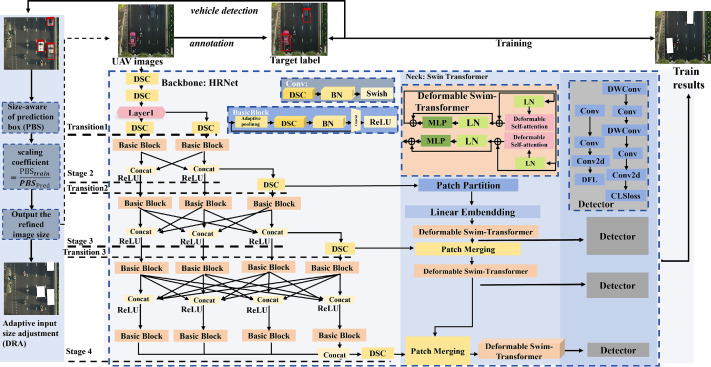
\includegraphics[width=.85\textwidth]{figures/ar_vdn.png}
    \caption{Arquitectura de la red AR-VDN\\
    \footnotesize{Fuente: \textit{https://www.sciencedirect.com/science/article/pii/S0926580526001342}}}
    \label{fig:ar-vdn}
\end{figure}



Leyre Encio et Al. \cite{articleEncio} proponen un sistema de detección de vehículos por la noche, un problema común debido a la falta de visibilidad tanto para los vehículos autónomos como para la gestión del tráfico. Este sistema que se adapta a las condiciones de iluminación, es una red neuronal basada en \textbf{CenterNet} (que a su vez se basa en CornerNet) y cuya arquitectura se divide en 2 bloques fundamentales: un backbone de CNNs y un bloque de detección. El backbone se basa en una arquitectura \textbf{Hourglass}, mostrada en la figura \ref{fig:hourglass}, seleccionada por su capacidad de \textbf{capturar detalles pequeños a múltiples escalas}. Esta arquitectura trata de asimilar un diseño de encoder-decoder, donde la imagen pasa a través de una serie de transformaciones hasta que acaba siendo un \textit{embedding} n-dimensional, al cual se le aumenta la resolución y termina con su tamaño original. Este sistema se ha probado en una CPU Intel Core i9-13900K \@ 5.8 GHz y 2 GPUs NVIDIA RTX 4090 de 24 GB. La evaluación se realizó usando tres datasets diferentes: \textbf{BDD100K}, \textbf{PVDN} y \textbf{FNTVD} \footnote{Este dataset es accesible a través de \url{https://www.gti.ssr.upm.es/data/ficosa}}. Los resultados obtenidos en los dos primeros datasets son los descritos en la tabla \ref{tab:bdd-pvdn}, y un rendimiento de \textbf{45 FPS}.

\begin{table}[htb]
    \centering
    \begin{tabular}{|c|c|c|}
         \hline   
         \textbf{Métrica} & \textbf{BDD100K} & \textbf{BVDN}\\
         \hline
         \textbf{mAP} & 71.34\% & 66.21\%\\ 
         \hline
         \textbf{F1-score} & 75.54\% & 73.74\%\\
         \hline
         \textbf{Precision} & 77.36\% & 79.49\%\\
         \hline
         \textbf{Recall} & 73.79\% & 68.76\%\\
         \hline
    \end{tabular}
    \caption{Resultados de la arquitectura con Hourglass en los datasets BDD100K y BVDN}
    \label{tab:bdd-pvdn}
\end{table}

\begin{figure}[htb]
\centering
    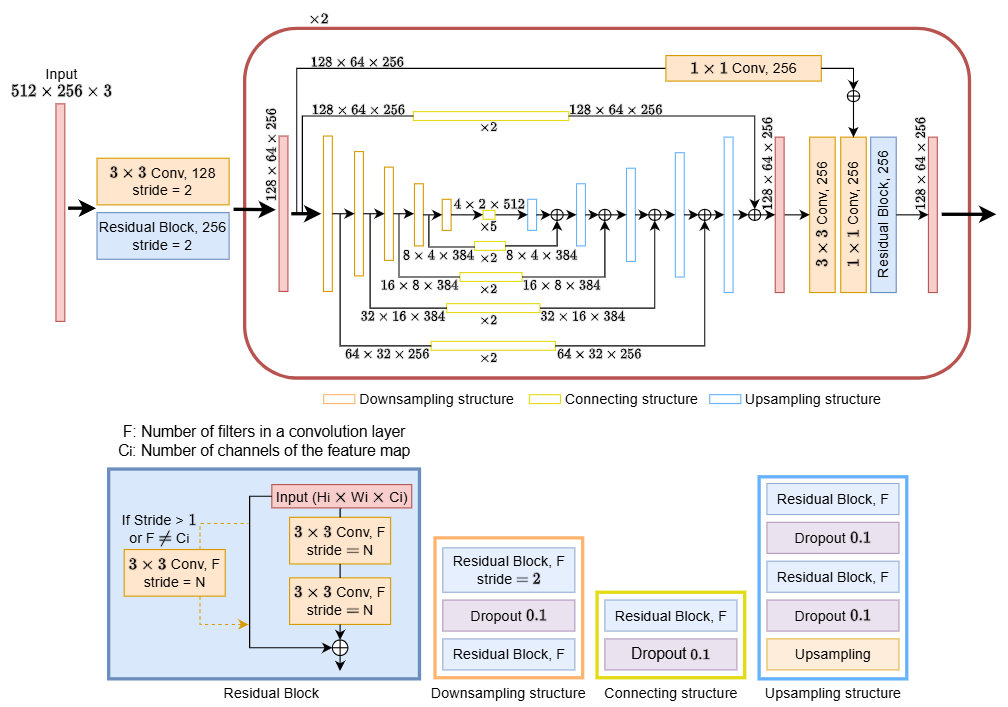
\includegraphics[width=.85\textwidth]{figures/hourglass.png}
    \caption{Arquitectura Hourglass\\
    \footnotesize{Fuente: \textit{https://www.researchgate.net/publication/389643765\_Enhanced\_Nighttime\_Vehicle\_Detection\_for\_On-board\_Processing}}}
    \label{fig:hourglass}
\end{figure}



De forma similar al artículo anterior, N.Jathin Reddy et Al. \cite{articleReddy} proponen un sistema de detección de vehículos preciso en entornos con baja visibilidad con el objetivo de ayudar a los sistemas inteligentes de transporte. Este problema puede deberse a una multitud de factores como el desenfoque de movimiento o el deslumbramiento por los faros de otros coches. La investigación propone usar la avanzada extracción de características y la arquitectura optimizada de \textbf{YOLOv10} para destacar en la precisión de detección, en la eficiencia computacional y en la solidez. Antes de entrenar el modelo, se aplican varias técnicas de preprocesado: ecualización adaptativa del histograma, reducción del ruido y mejora del contraste. Los experimentos producidos demuestran que \textbf{YOLOv10} tiene un rendimiento superior en las métricas de mean Average Precision (mAP), velocidad de inferencia y reducción de falsos positivos comparando con otros modelos como YOLOv8 y Faster R-CNN.



Este siguiente trabajo de Liang Liang et Al. \cite{s24103088} contribuye con un amplio estudio de tecnologías existentes en la tarea de detección de vehículos, proporcionando una descripción breve de las tareas, las métricas y los datasets en primer lugar. En segundo lugar, más de 200 algoritmos, tanto clásicos como novedosos, han sido resumidos detalladamente. En cuanto a los algoritmos de detección se pueden dividir en 3 tipos, distinguibles en la figura \ref{fig:detection-methods}:
\begin{itemize}
    \item[Anchor-based]: \textbf{Las bounding boxes predefinidas se usan para detectar los objetos}. Dependiendo de si se utilizan propuestas de regiones, este tipo de detectores se dividen a su vez en dos:
    \begin{itemize}
        \item[Two-stage]: \textbf{Se generan las propuestas de región y luego se hace la clasificación y la regresión de los puntos de interés}. Los modelos \textbf{R-CNN}, \textbf{SPP-Net}, \textbf{R-FCN}, \textbf{FPN} y \textbf{Cascade R-CNN} son algunos ejemplos comunes. Faster R-CNN consiste en una red de propuestas de región diferente al resto. Este tipo de métodos refinan muchas veces los anclajes (anchors) lo que resulta en detecciones más precisas.
        \item[One-stage]: Predice el centro y las bounding boxes de los vehículos colocando anclajes en el mapa de características. Algunos detectores incluyen \textbf{SSD}, \textbf{M2Det}, \textbf{RetinaNet} y la serie de modelos \textbf{YOLO} desde YOLOv2 hasta YOLOv7. A pesar de sacrificar algo de precisión en la detección, tienen una ventaja considerable en términos de inferencia.
    \end{itemize}
    \item[Anchor-free]: Este tipo de modelos \textbf{predicen el centro o los puntos clave de un objeto} y los agrupa para obtener la \textit{bounding box}. El acercamiento por puntos clave supone detectar características clave del objeto para determinar su posición y forma. Entre los modelos se encuentran \textbf{CornerNet}, \textbf{RepPoints}, \textbf{CenterNet}, \textbf{ExtremeNet} y \textbf{Grid R-CNN}. Algunos modelos clásicos que se basan en el centro del objeto son \textbf{YOLOv1}, \textbf{FSAF}, \textbf{FCOS}, \textbf{GA-RPN}, \textbf{FoveaBox}, \textbf{YOLOX}, \textbf{YOLOv8} y \textbf{YOLOv9}.
    \item[End-to-end]: Los anteriores métodos predicen un conjunto de bounding boxes a través de regresión y clasificación. Los detectores \textit{end-to-end} \textbf{determinan la posición y clase de un objeto sin aplicar procedimientos adicionales de preprocesado y/o posprocesado}. Aquí se incluyen los modelos \textbf{DeFCN}, \textbf{Sparse R-CNN} o \textbf{DETR}, el cual utiliza una red neuronal basada en transformadores. 
    \end{itemize}

\begin{figure}[htb]
\centering
    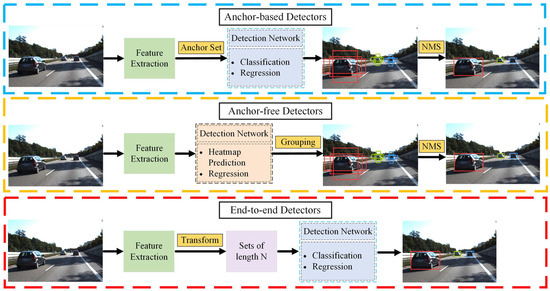
\includegraphics[width=.85\textwidth]{figures/detection_methods.png}
    \caption{Funcionamiento de distintos métodos de detección de vehículos\\
    \footnotesize{Fuente: \textit{https://www.mdpi.com/1424-8220/24/10/3088}}}
    \label{fig:detection-methods}
\end{figure}





% --------------------
\section{Métodos seleccionados}
% --------------------
\label{sec:selectedMethod}

\subsection{YOLOv26n}

YOLO26 \cite{sapkota2026yolo26keyarchitecturalenhancements}, publicado en Septiembre de 2025, es la versión más novedosa entre los modelos YOLO, con más mejoras en cuestión de eficiencia, precisión y despliegue en dispositivos de menor rendimiento; algo que se puede observar en la figura \ref{fig:yolo-stats}. 

\begin{figure}[htb]
\centering
    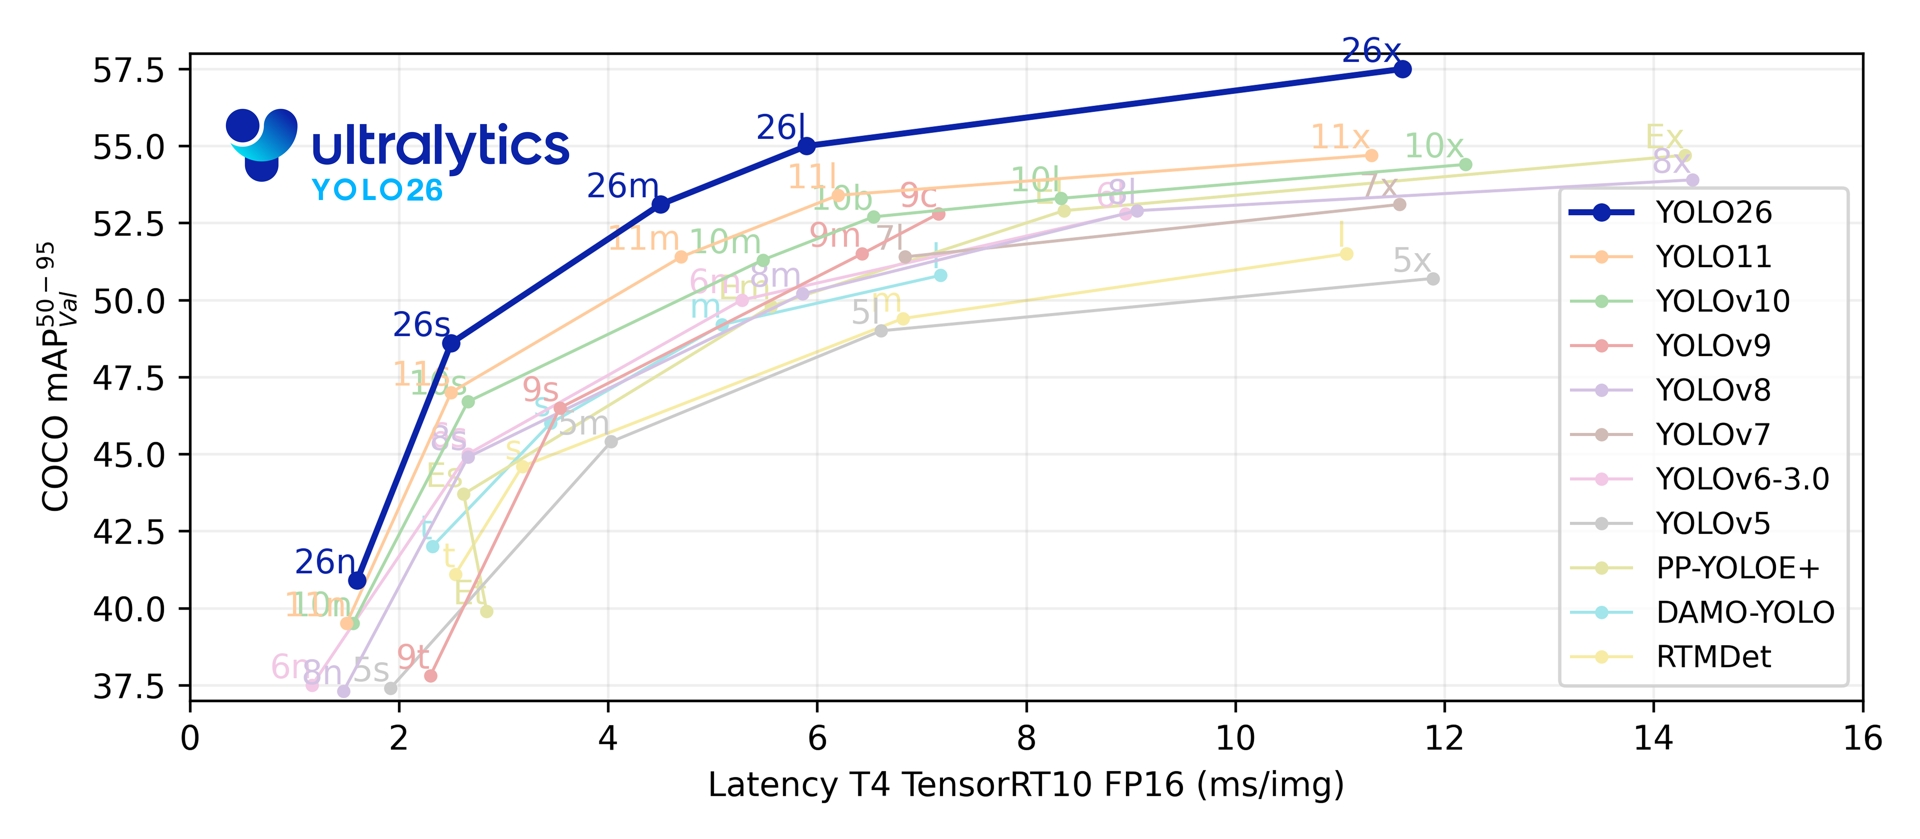
\includegraphics[width=.85\textwidth]{figures/yolo_stats.png}
    \caption{Compensación entre velocidad y precisión entre los distintos modelos YOLO\\
    \footnotesize{Fuente: \textit{https://arxiv.org/pdf/2509.25164}}}
    \label{fig:yolo-stats}
\end{figure}

\subsubsection{Arquitectura de YOLO26}

Esta nueva arquitectura, visible en la figura \ref{fig:yolo26-arch}, elimina el \textit{Distribution Focal Loss} (DFL) \footnote{Función de pérdida que cuantifica el objetivo de la regresión en múltiples celdas o contenedores, permitiendo que sea más flexible la representación de las \textit{bounding boxes}.} e integrando \cite{chakrabarty2026yolo26analysisnmsfreeend}:

\begin{figure}[htb]
\centering
    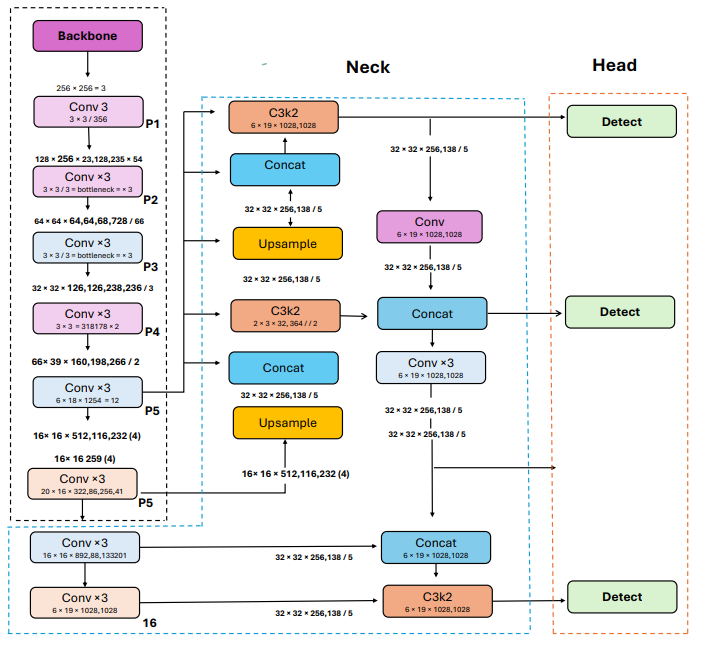
\includegraphics[width=.85\textwidth]{figures/yolo26_arch.png}
    \caption{Arquitectura del modelo YOLO26 para detección y segmentación\\
    \footnotesize{Fuente: \textit{https://arxiv.org/pdf/2509.25164}}}
    \label{fig:yolo26-arch}
\end{figure}

\begin{itemize}
    \item \textbf{NMS-Free inference End to End:} NMS es una función que elimina \textit{bounding boxes} superpuestas a otras, seleccionando la propuesta con mayor confianza. YOLO26 rediseña la predicción, haciendo que el modelo prediga \textbf{una sola bounding box por cada instancia} durante el entrenamiento. Eliminar esta parte \textbf{mejora en un 43\% la latencia} en el entrenamiento con el uso de la CPU, en donde se hacía un cuello de botella debido a multitud de operaciones secuenciales.
    
    \item \textbf{ProgLoss:} Es una estrategia de pérdida de pesos dinámica. En otros detectores, tiene que haber un balance entre el arreglo por la función de pérdida de clasificación ($L_{cls}$) y el arreglo por la función de pérdida de regresión de la \textit{bounding box} ($L_{box}$), lo que provoca que la red neuronal tenga que aprender a la vez a diferenciar entre características y a localizar con precisión sin el uso de anclajes. 
    
    Este nuevo sistema introduce un coeficiente $\lambda_t$ en la ecuación: 
    \begin{equation*}
        L_{total}(t) = \lambda_t * L{cls} + (1 - \lambda_t) * L_{box}
    \end{equation*}
    lo que resulta en que el aprendizaje prioriza las \textbf{características de alto nivel al principio} del entrenamiento y, \textbf{según progresa el aprendizaje}, este va priorizando \textbf{características geométricas de grano fino}, lo que se puede observar en la figura \ref{fig:progloss}.

    \begin{figure}[htb]
    \centering
        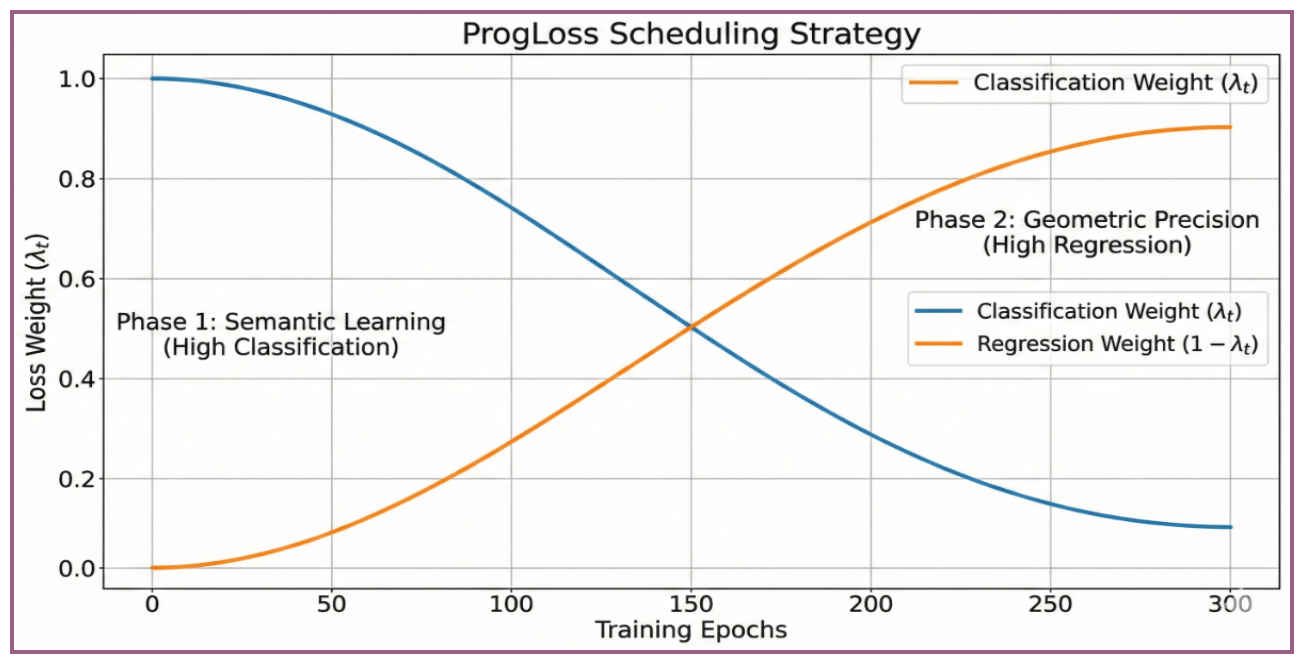
\includegraphics[width=.85\textwidth]{figures/progloss.png}
        \caption{Estrategia de priorización del sistema Progloss\\
        \footnotesize{Fuente: \textit{https://arxiv.org/html/2601.12882v1}}}
        \label{fig:progloss}
    \end{figure}


    \item \textbf{Small-Target-Aware Label Assignment:} STAL es una implementación que nace para solucionar el problema "desvanecimiento del objeto pequeño", donde la dependencia del umbral de IoU de estrategias típicas no funciona en objetos pequeños (ocupando menos de un 1\% de la imagen) debido a la sensibilidad del IoU a pequeñas traslaciones espaciales. STAL, como se define en la siguiente ecuación:     
    
    \begin{equation*}
        \tau_{dynamic} = \tau_{base} * (1 - \alpha * \varepsilon^{-\frac{Area_{obj}}{Area_{img}}})
    \end{equation*}
    
    reemplaza el umbral fijo, que suele ser en torno a 0.5, por un umbral $\tau$ que se reduce según el tamaño del objeto y un parámetro $\alpha$ para la tasa de decaimiento en la que el umbral se reduce.

    \item \textbf{Optimizador MuSGD:} Debido a la eliminación del módulo DFL, es necesario introducir un entrenamiento más robusto que no permita que el descenso del gradiente colapse. Ultralytics introduce a YOLO26 el optimizador MuSGD, un optimizador híbrido que fusiona las propiedades del SGD estándar con el optimizador Muon. Este último realiza una ortogonalización matricial, actualizando la matriz de pesos para que sea ortogonal a su estado actual.

    Definimos el \textit{buffer} del momento estándar $v_t$ usado en SGD
    
    \begin{equation*}
        v_{t+1} = \beta * v_t + g_t
    \end{equation*}
    
    donde $g_t$ es el gradiente y $\beta$ es el coeficiente del momento. MuSGD modifica la última actualización de los pesos usando la \textbf{ortogonalización de Newton-Schulz} \footnote{En lugar de expandir polinomios largos y repetir multiplicaciones sobre dimensiones extensas, se agrupa el proceso iterativo en una estructura unificada que evalúa la contribución real de cada potencia matricial. Al identificar y eliminar términos de escasa relevancia y al permitir que algunos coeficientes sean aprendidos por optimización, se consigue una combinación más parsimoniosa que converge de forma más estable y con menos operaciones pesadas \cite{q2bstudioUNSOOrtogonalizacixF3n}.}, la cual "blanquea" la matriz de gradientes usando un proceso iterativo de refinamiento: 
    \begin{equation*}
        \theta_{t+1} = \theta_t - \eta * (\alpha * v_{t+1} + (1 - \alpha) * NewtonSchulz(g_t))
    \end{equation*}
    Este método \textbf{mitiga la varianza} de SGD mientras \textbf{elimina la inestabilidad de las actualizaciones ortogonales} de Muon: figura \ref{fig:musgd}.

    \begin{figure}[htb]
    \centering
        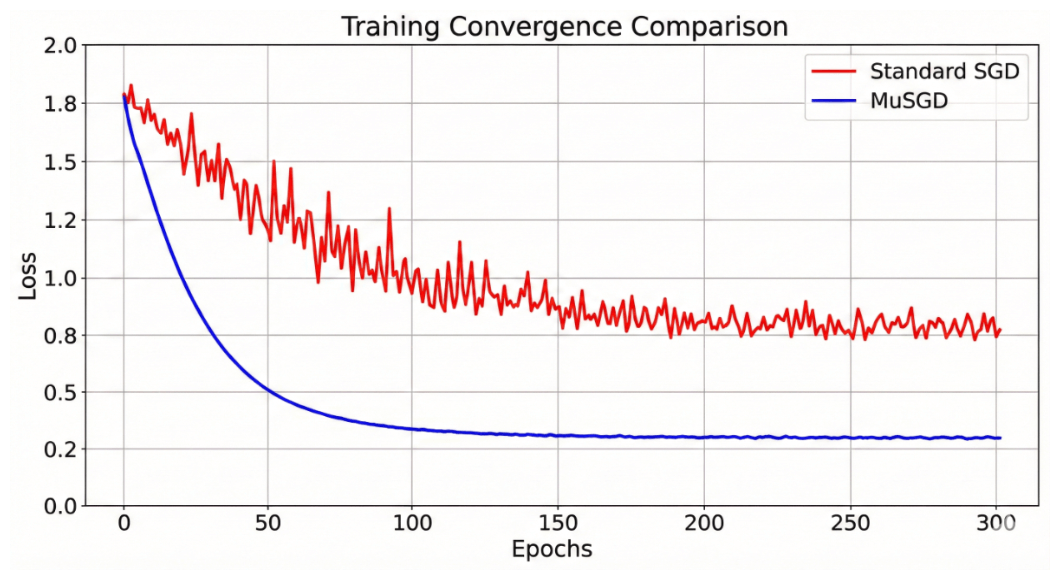
\includegraphics[width=.85\textwidth]{figures/musgd.png}
        \caption{Concepto visual esperado de la optimización dinámica de MuSGD\\
        \footnotesize{Fuente: \textit{https://arxiv.org/html/2601.12882v1}}}
        \label{fig:musgd}
    \end{figure}
\end{itemize}



\subsubsection{Modelos}

Aunque YOLO se creó con la principal finalidad de la tarea de detección, se han ido creando distintos modelos a lo largo de las versiones de YOLO con diferentes fines: clasificación, segmentación de instancias, detección de puntos claves/poses y detección de objetos orientados. Actualmente, Ultralytics construye 5 modelos distintos con la misma estructura, aunque con diferentes tamaños de capas. Para esta última versión de detección de YOLO, YOLO26, hay 5 modelos más o menos potentes (dependiendo del número de parámetros), cuyas especificaciones se pueden observar en la tabla \ref{tab:yolo-models} usando imágenes de 640 x 640 píxeles, redimensionadas del conjunto de datos COCO.

\begin{table}[htb]
    \centering
    \begin{tabular}{c|c|c|c|c}
        \hline
        \textbf{Modelo} & \textbf{mAP}$\_{val}$\textbf{50-95} & \textbf{Velocidad T4 TRT10(ms)} & \textbf{Parámetros(M)} & \textbf{FLOPs(B)}\\
        \hline
        \textbf{YOLO26n} & 40.9\% & 1.7 ms & 2.4 M & 5.4 B\\
        \hline
        \textbf{YOLO26s} & 48.6\% & 2.5 ms & 9.5 M & 20.7 B\\
        \hline
        \textbf{YOLO26m} & 53.1\% & 4.7 ms & 20.4 M & 68.2 B\\
        \hline
        \textbf{YOLO26l} & 55.0\% & 6.2 ms & 24.8 M & 86.4 B\\
        \hline
        \textbf{YOLO26x} & 57.5\% & 11.8 ms & 55.7 M & 193.9 B\\
        \hline
    \end{tabular}
    \caption{Resultados de los distintos modelos YOLO26 de detección}
    \label{tab:yolo-models}
\end{table}


\subsection{DINO-DETR}

DINO-DETR \cite{zhang2022dino} es un detector de objetos end-to-end que mejora anteriores modelos basados en el modelo DETR \cite{DBLP:journals/corr/abs-2005-12872} en términos de rendimiento y eficiencia usando un método contrastativo para eliminar ruido en el entrenamiento, selección de consultas mixtas para inicializar los puntos clave y un esquema \textit{"look forward twice"} para predecir las \textit{bounding boxes}. Este modelo logra alcanzar un 49.4 de AP en 12 iteraciones y un 51.3 en 24, mejorando en 6.0 y 2.7, respectivamente al modelo DN-DETR. Este modelo se encuentra disponible a través de: \url{https://github.com/IDEA-Research/DIN}. 


\subsection{DFEM-Net}
\url{https://github.com/ahtarv/DFEM-Net}









% --------------------
\section{Datasets}
\label{sec:datasets}
% --------------------

Se han investigado y recopilado varios conjuntos de datos desde varias fuente, sobre todo desde Kaggle y Github. Los mejores datasets para el proyecto tendrían que tener tanto imágenes del mismo vehículo desde diferentes ángulos/cámaras como que la matrícula sea legible. Lamentablemente, el tipo de datasets que cumplan ambas funciones son bastante raros, aunque se han podido sacar 2 datasets que lo cumplen y otros dos que, aunque no hay posibilidad de variedad de cámaras hacia el mismo objetivo, aportan con gran cantidad de vehículos y sus matrículas.



\subsection{Multi-perspective traffic video analysis}

Este conjunto de datos \cite{Sanchez-Iborra2026} está comprendido por 3 escenarios distintos, las cuales a su vez se dividen en 3 perspectivas distintas (cámara del coche, dron y cámara de vigilancia), que a su vez cada una se divide en 2 secuencias de vídeo distintas grabadas a una resolución de \textbf{1920 x 1080} a \textbf{60 fotogramas por segundo}; el total de secuencias de vídeo alcanzando 18. Un ejemplo de fotograma del dataset se puede observar en la figura \ref{fig:rsu-esc1}. Ya que este conjunto de datos no lleva ninguna etiqueta asociada a alguno de los vídeos, se utilizará únicamente para el conjunto de pruebas.

\begin{figure}[htb]
\centering
    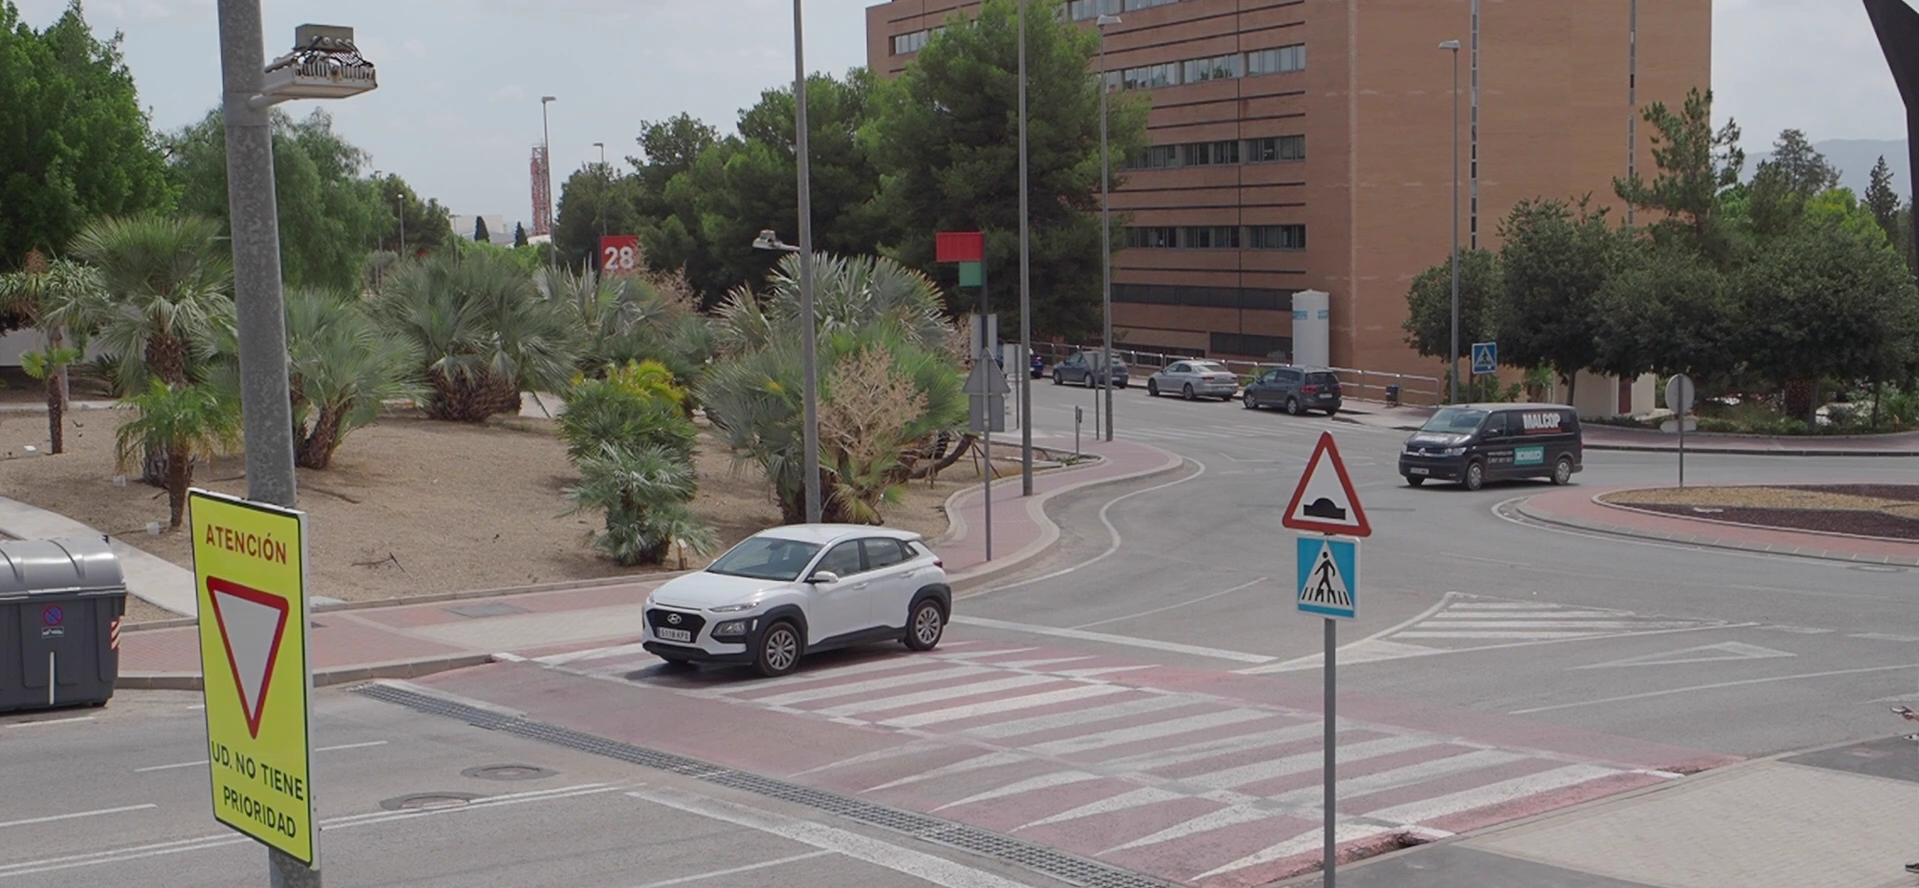
\includegraphics[width=.85\textwidth]{figures/rsu_esc1.png}
    \caption{Fotograma del escenario 1 con la perspectiva de una RSU\\
    \footnotesize{Fuente: \textit{https://zenodo.org/records/18375218}}}
    \label{fig:rsu-esc1}
\end{figure}



\subsection{Bdd100k}

Este conjunto de datos \cite{bdd100k} es uno de los más grandes y diversos en cuestión de imágenes de vehículos con anotaciones precisas. Como sugiere el nombre, el dataset consta de 100,000 vídeos grabados desde una cámara acoplada en la parte delantera interior del vehículo; cada uno dura 40 segundos y están grabados a una resolución de \textbf{720 píxeles} a \textbf{30 fps}. Para mantener un dataset diverso, Bdd100k cubre diferentes condiciones climáticas y periodos del día. Las anotaciones incluyen tanto las de detección como las de segmentación y cubren 10 categorías diferentes, como los autobuses y las señales, pudiéndose observar en la figura \ref{fig:bdd} el número de apariciones de cada una de ellas en el dataset. Un ejemplo del conjunto de datos se puede observar en la figura \ref{fig:bdd-example}. Este conjunto de datos se utilizará inicialmente para entrenar y validar (para que el modelo se adapte bien a nuevos datos) los modelos.

\begin{figure}[htb]
\centering
    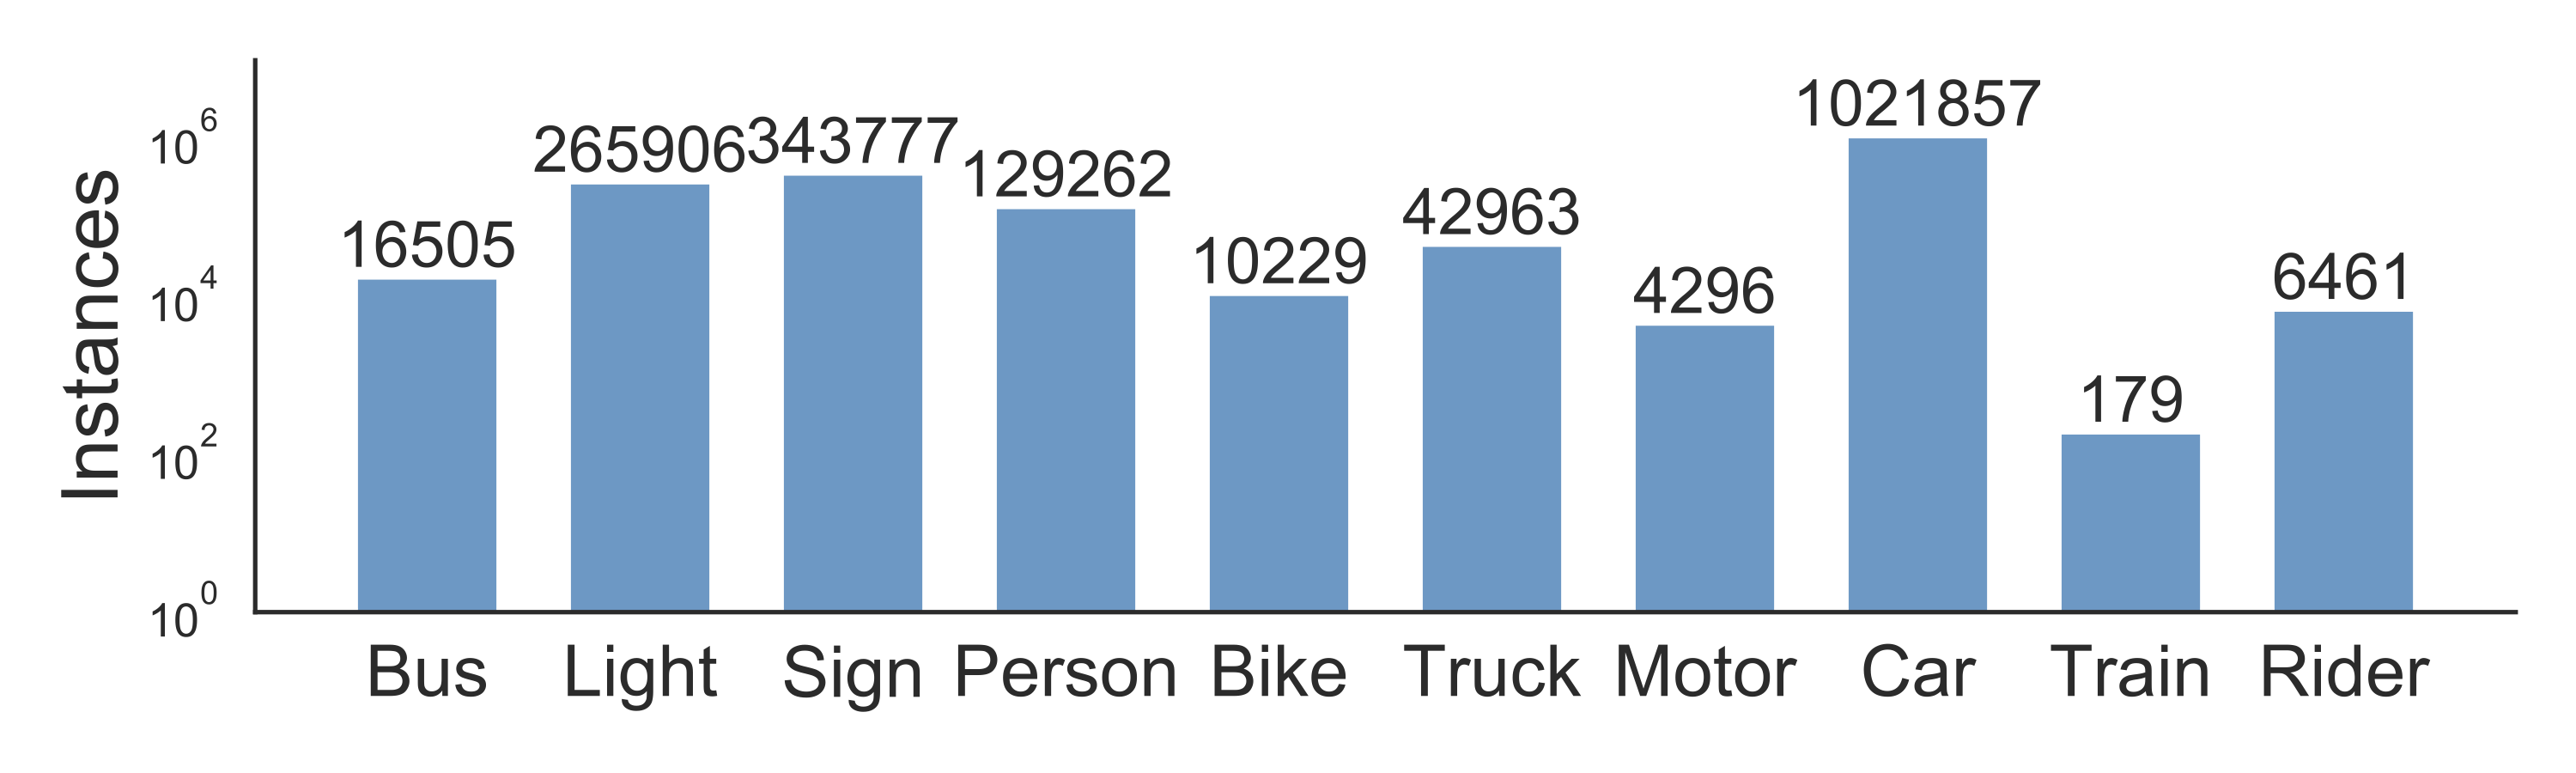
\includegraphics[width=.85\textwidth]{figures/bdd100k.png}
    \caption{Estadísticas de los diferentes tipos de objetos en el dataset Bdd100k\\
    \footnotesize{Fuente: \textit{https://bair.berkeley.edu/blog/2018/05/30/bdd/}}}
    \label{fig:bdd}
\end{figure}

\begin{figure}[htb]
\centering
    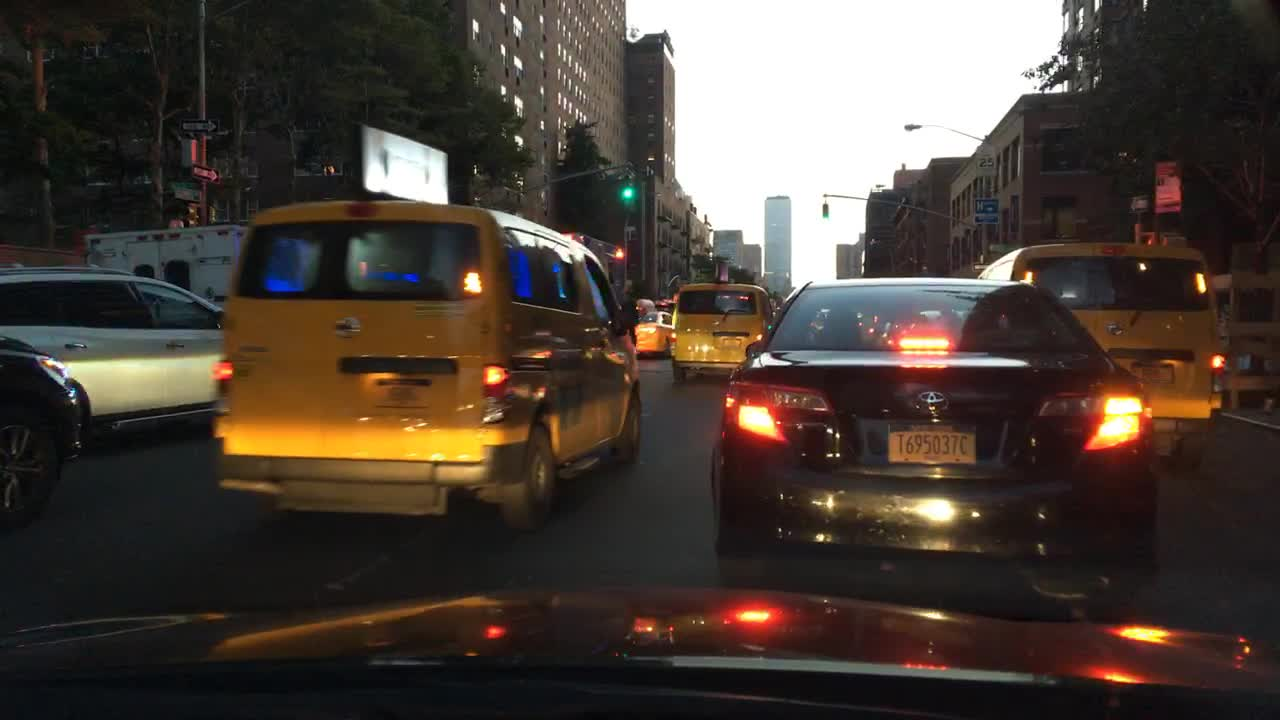
\includegraphics[width=.85\textwidth]{figures/bdd_example.png}
    \caption{Ejemplo del dataset Bdd100k\\
    \footnotesize{Fuente: \textit{https://www.kaggle.com/datasets/solesensei/solesensei\_bdd100k}}}
    \label{fig:bdd-example}
\end{figure}



\subsection{UC3M-LP}

Este conjunto de datos creado por investigadores de la universidad Carlos III de Madrid \cite{RAMAJOBALLESTER2024104608} es presentado para la tarea de \textbf{detección de matrículas y reconocimiento de caracteres} junto a otro dataset de gran tamaño para reidentificación de vehículos: UC3M-VRI. Se almacenan 1975 imágenes de 2547 vehículos distintos, lo que hacen 2547 matrículas, sumando un total de 12757 caracteres. Algunos ejemplos se pueden observar en la figura \ref{fig:uc3mlp-example}. La variedad de imágenes es amplia en cuestión de luz: 2185 imágenes de día y 362 de noche; la distancia de la cámara al vehículo es de entre 1 y 20 metros y la perspectiva cambia en cada imagen. El conjunto se ha probado en diferentes modelos de detección, incluyendo varias arquitecturas YOLO (varios modelos de los YOLOv3, YOLOv4 y YOLOv5), EfficientDet, ATSS y ASFF, siendo el resultado más notable el de \textbf{YOLO5s} con un tamaño de imagen de \textbf{1280 píxeles}, consiguiendo un \textbf{mAP@0.5 de 98.8\%} y un \textbf{mAP@0.5-0.95 de 89.3\%}. En el caso del reconocimiento de la matrícula, utilizando el mismo modelo con el tamaño de imagen de \textbf{640 píxeles y el optimizador AdamW} se consigue un \textbf{mAP@0.5 de 97.6\%} y un \textbf{mAP@0.5-0.95 de 76.4\%}.

\begin{figure}[htb]
\centering
    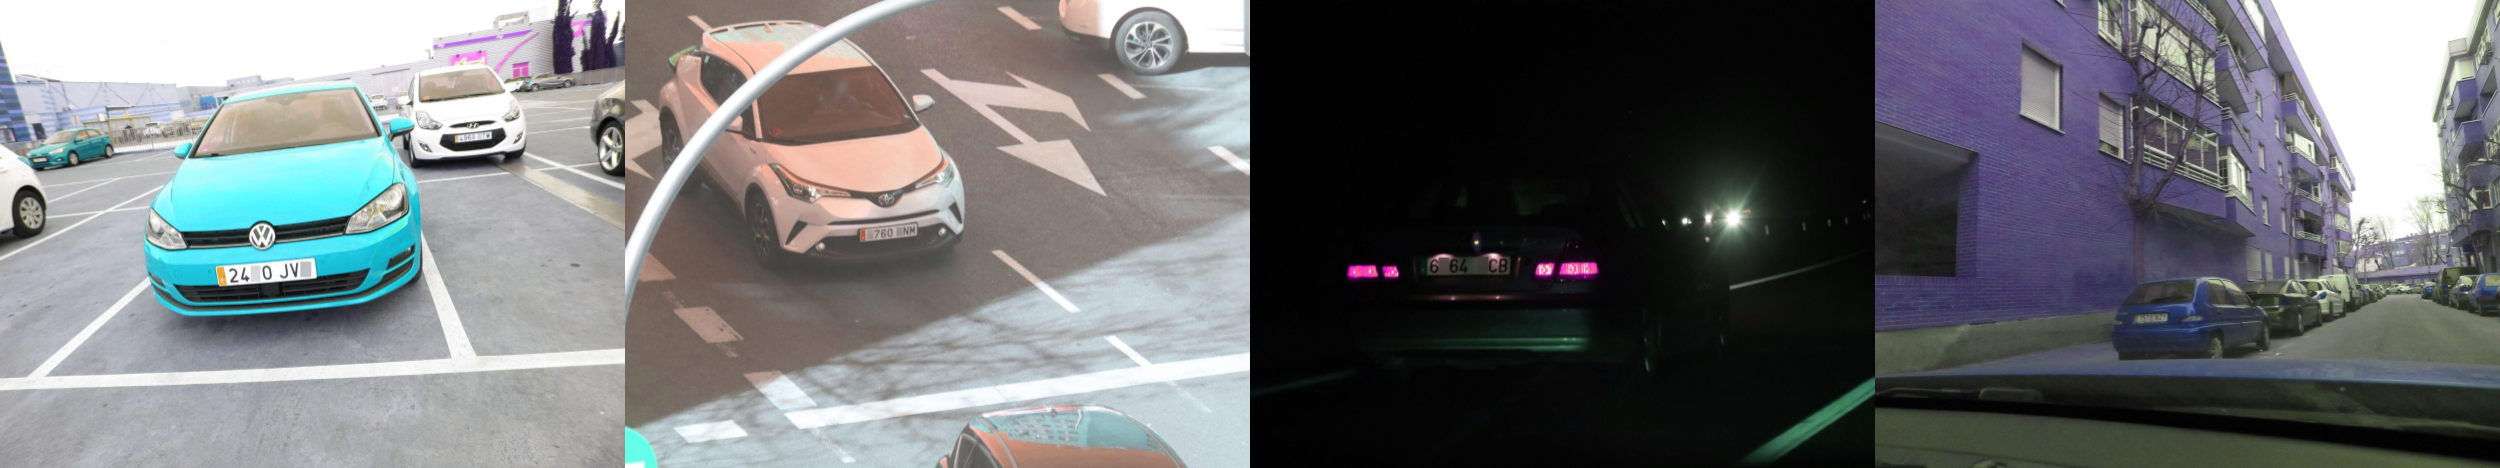
\includegraphics[width=.85\textwidth]{figures/uc3mlp_example.png}
    \caption{Ejemplos del dataset UC3M-LP\\
    \footnotesize{Fuente: \textit{https://github.com/ramajoballester/UC3M-LP}}}
    \label{fig:uc3mlp-example}
\end{figure}



\subsection{UC3M-VRI}

Este conjunto de datos es la otra mitad de la investigación del dataset anterior \cite{RAMAJOBALLESTER2024104608} y está orientado a reidentificación de vehículos. Se almacenan 1611 imágenes de 286 vehículos distintos todas sacadas de día y divididas en dos subconjuntos:
\begin{itemize}
    \item \textbf{Conjunto de carretera:} 458 imágenes de 201 vehículos diferentes, sacadas a una distancia de entre 5 a 7 metros con una sola perspectiva.
    \item \textbf{Conjunto de intersección:} 1153 imágenes de 85 vehículos diferentes, sacadas a una distancia de entre 10 y 20 metros usando 2 cámaras para realizar diferentes planos sobre los vehículos que aparecen.
\end{itemize}
Algunos ejemplos se pueden observar en la figura \ref{fig:uc3mlp-example}. Los modelos seleccionados son EfficientNetB0 y FastReid, cada uno con otros 2 modelos que han sido entrenados en datasets diferentes: \textbf{Stanford-Cars} \cite{6755945}, \textbf{VeRi-776} y \textbf{VeRi-Wild}. El modelo con mayores resultados ha sido FastReid (entrenado en VeRi-776) con un 97.9\% de accuracy con el test positivo-negativo (se selecciona una imagen (positiva) y se selecciona una segunda del resto de clases (negativa)) en el subdataset de carreteras y un 87.8\% de accuracy en el subdataset de intersecciones.

\begin{figure}[htb]
\centering
    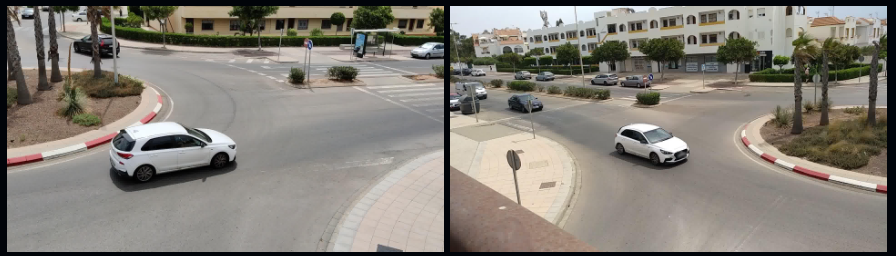
\includegraphics[width=.85\textwidth]{figures/uc3mvri_example.png}
    \caption{Ejemplos del dataset UC3M-VRI\\
    \footnotesize{Fuente: \textit{https://github.com/ramajoballester/UC3M-VRI}}}
    \label{fig:uc3mvri-example}
\end{figure}





% --------------------
\section{Métricas}
% --------------------
\label{sec:metrics}
Para poder validar de forma equitativa los distintos métodos, se tienen que seguir unas métricas a seguir para todos. Para empezar, se tiene que hablar del tiempo de procesamiento por imagen, ya que la velocidad de inferencia es prioritaria a la hora de detectar y reconocer claramente el vehículo y su matrícula.

\begin{itemize}
    \item \textbf{mAP50}: Precisión media de las detecciones, calculada con un umbral de intersección (IoU) de 0,5.

    \item \textbf{mAP50-95}: Media entre todas las precisiones medias entre el umbral IoU 0,50 y 0,95, ambos umbrales incluidos.

    \item \textbf{Precisión}: En una clase, es el número de predicciones correctas para esta clase entre el número total de predicciones para esta misma clase.

    \item \textbf{Recall}: En una clase, es el número de predicciones correctas para esta clase entre el número total de instancias de esta misma clase.

    \item \textbf{F1-score}: Es una métrica especializada para cuando las clases están desbalanceadas, es decir, el número de instancias de cada clase no es el mismo para cada una. Se calcula primero para cada clase con la ecuación:
    \begin{gather*}
        F1score = 2 \times \dfrac{Precision \times Recall}{Precision + Recall}
    \end{gather*}
\end{itemize}

En el caso de las métricas de Precision, Recall y F1-score, para hacer la media del dataset entero hay dos opciones: (1) \textbf{Macro}: El sumatorio del \textit{f1-score} de cada clase entre el número de clases y (2) \textbf{Ponderada}: Considerar el número de instancias de cada clase, siendo las clases con mayor número de imágenes las que más aportan a la media.


% --------------------
\section{Metodología experimental}
\label{sec:met-exp}
% --------------------

La metodología que se ha empleado es la habitual en el desarrollo de programas relacionados con \textit{Machine Learning} y/o \textit{Deep Learning}, similar al de la figura \ref{fig:metodologia-dl}: (1) Recogida de datos, (2) Procesamiento de los datos, (3) Selección de los modelos, (4) Entrenamiento de los modelos, (5) Validación del modelo y resultados.

\begin{figure}[htb]
\centering
    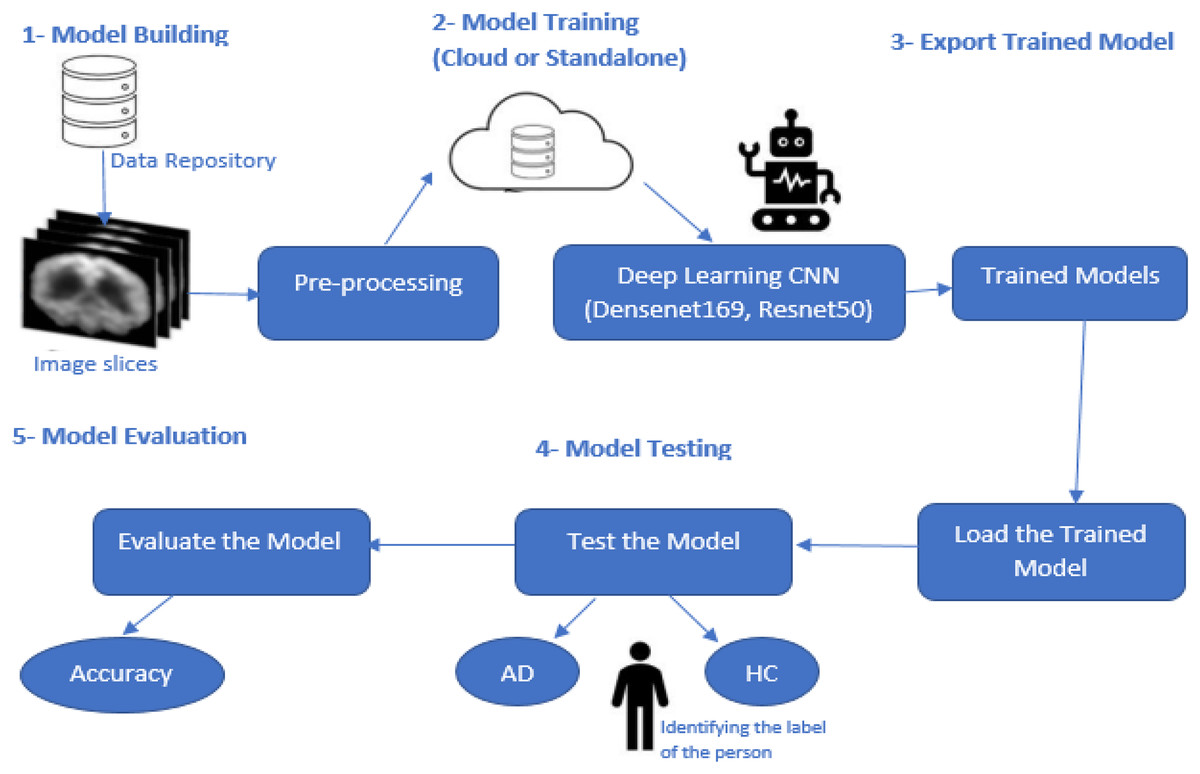
\includegraphics[width=.85\textwidth]{figures/methodology_dl.jpg}
    \caption{Metodología del diagnóstico y clasificación de Alzheimer con CNNs\\
    \footnotesize{Fuente: \textit{https://peerj.com/articles/cs-1177/}}}
    \label{fig:metodologia-dl}
\end{figure}


\subsection{Extracción y estructuración de los datos}

%[TODO] Despues de seleccionar el/los dataset/s, introducirlo/s con su propia estructura, tamaño de imagen, etiquetas, división...

Ya que el modelo YOLO necesita un estructurado concreto, lo primero es construir un programa personalizado que ...

La estructura del conjunto de datos que tiene que seguir YOLO es de la siguiente forma:
% \dirtree{%
%     .1 *.py.
%     .1 datasets.
%     .2 test.
%     .2 train.
%     .2 val.
%     .3 images.
%     .4 labels.
% }

\subsection{Preprocesado de datos}


\subsection{Entrenamiento}

En este apartado se mostrarán los diferentes parámetros y configuraciones aplicadas o que se han probado en los entrenamientos de los modelos.


\subsubsection{YOLO}

Gracias a Ultralytics \footnote{Toda la información de la librería de Ultralytics es de código abierto y está disponible en \url{https://github.com/ultralytics/ultralytics}}, está a disposición de estudiantes e investigadores una librería entera con montones de recursos para poder entrenar, validar y probar los modelos YOLO. De entre todos los parámetros disponibles, para el entrenamiento de este modelo se han utilizado o experimentado con los siguientes:

\begin{itemize}
    \item \textbf{Model}: Modelo que será entrenado.

    \item \textbf{Epochs}: Cada época representa una pasada por el dataset entero.
    
    \item \textbf{Time}: Tiempo máximo del entrenamiento. Si este campo no está vacío, se usará en vez del parámetro de las iteraciones.

    \item \textbf{Batch}: El tamaño de lote significa el número de datos de entrenamiento procesadas por el modelo en una sola iteración. En vez de procesarse el dataset entero, este se divide en unos grupos de datos o \textit{batches}.

    \item \textbf{Device}: Especifica si se quiere usar la \textbf{CPU}, una única \textbf{GPU} o múltiples \textbf{GPUs} para maximizar la eficiencia del modelo y tardar mucho menos en este proceso.

    \item \textbf{Workers}: Número de hilos trabajadores para la carga de datos. Influye especialmente en la velocidad del procesamiento si se está usando la \textit{GPU}.

    \item \textbf{Optimizer}: Escoger el optimizador para el entrenamiento entre \textbf{SGD}, \textbf{Adam}, \textbf{AdamW}, etc. Afecta a la estabilidad y a la velocidad de convergencia. Por defecto, se selecciona por sí solo en función del modelo.

    \item \textbf{Cos\_lr}: Se utiliza un \textit{scheduler} o programador de la tasa de aprendizaje coseno, ajustando la tasa de aprendizaje siguiendo una curva coseno a lo largo de los \textit{epochs} para mejorar la convergencia.

    \item \textbf{Freeze}: Número de primeras capas del modelo a congelar para reducir el número de parámetros entrenables.

    \item \textbf{Lr0}: Tasa de aprendizaje inicial, influye en la rapidez con la que se actualizan los pesos del modelo.

    \item \textbf{Lrf}: Factor de la tasa de aprendizaje, que sirve junto a la tasa de aprendizaje inicial, para calcular la tasa de aprendizaje final de la forma: $lr\_final = lr0 \times lrf$. Se usa en conjunto con el \textit{scheduler} (como el coseno) para ajustar la tasa de aprendizaje a lo largo del entrenamiento.

    \item \textbf{Weight decay}: Valor de regularización L2, que penaliza los pesos grandes para evitar que el modelo se sobreajuste a los datos de entrenamiento (overfitting).

    \item \textbf{Dropout}: Tasa de pérdida de nodos del modelo para la regularización en tareas de clasificación, que evita el sobreajuste omitiendo aleatoriamente unidades durante el entrenamiento.

    \item \textbf{Cache}: Decide si se quiere guardar en memoria RAM o disco las imágenes del conjunto de datos. Mejora la velocidad de entrenamiento a costa de un mayor uso de memoria.

    \item \textbf{Data}: Archivo de configuración del dataset con formato \textit{.yaml}. En este archivo se fijan las rutas a las carpetas de entrenamiento, validación y pruebas, el número de clases y la asignación de IDs a cada clase. El archivo usado para entrenar el modelo YOLO se puede observar en la figura %\ref{fig:yaml}.

    \item \textbf{Imgsz}: Tamaño de imagen usado en el entrenamiento. Si las imágenes del conjunto de datos no están a este tamaño se redimensionan antes de introducirlas en el modelo.

    \item \textbf{Patience}: Número de etapas que hay que esperar antes de parar el entrenamiento durante las cuales las métricas de validación no mejoran.

    \item \textbf{Plots}: Dibujar gráficas de las métricas de entrenamiento y validación al acabar de entrenar el modelo. Además, se guardan varias imágenes con las predicciones hechas por el modelo YOLO para comprobar su rendimiento. 

    \item \textbf{Exist\_ok}: Decidir si se sobrescribe la carpeta donde se guardan los archivos de entrenamiento.
    
    \item \textbf{Save}: Decide si se guardan los pesos durante el entrenamiento para fijar puntos de control temporales. Esto permite resumir el entrenamiento a posteriori
    
    \item \textbf{Save\_period}: Cada cuántas épocas se realiza el guardado de pesos.

    \item \textbf{Single\_cls}: El modelo trata todas las clases del archivo de configuración como una sola. Es útil para centrar al modelo en solamente la tarea de detección.
    
    \item \textbf{Project}: Nombre del directorio donde se guardarán los resultados de entrenamiento.
\end{itemize}


\subsection{Rastreo del Overfitting}

Con el objetivo de evaluar el rendimiento del modelo y detectar posibles indicios de sobreajuste durante el entrenamiento, se ha realizado un seguimiento detallado de los valores de pérdida (loss\_rates), los cuales se registraron durante el entrenamiento en cada iteración en los conjuntos de entrenamiento y validación. El análisis de estas gráficas permite observar el comportamiento del modelo y determinar si está memorizando los datos de entrenamiento en lugar de generalizar correctamente.

En los experimentos realizados se ha prestado especial atención a la diferencia entre las pérdidas tanto de entrenamiento como de validación ya que dependiendo del diferencial entre ellas podría llevar al sobreajuste.



% --------------------
\section{Implementaciones en Python}
% --------------------
\label{sec:python}

Todo el desarrollo de las prácticas se subirá al siguiente repositorio de \textbf{GitHub}:\\ \url{https://github.com/RubenFdezGlez/MURIA-Practicas}. 

Este repositorio incluirá, además del código necesario para la ejecución del sistema, un \textbf{README} detallado con información sobre la implementación y la guía de instalación del programa.





% --------------------
\section{CREDITS}
% --------------------
\label{sec:credits}
Review the following link for your information: \footnote{https://www.elsevier.com/researcher/author/policies-and-guidelines/credit-author-statement} “CRediT (Contributor Roles Taxonomy) was introduced to recognize individual author contributions, reducing authorship disputes and facilitating collaboration”. More informally, it is a paragraph usually introduced at the end of research papers that recognizes the individual work of each author. You will see this in most of the papers you will be reviewing. 

The group will include a paragraph like the CRediT statement indicating who collaborated on each section and task of the research proposal. Not all the original CRediT Terms would be applicable, so the group could use the following:

\begin{table}[ht]
\centering
\begin{tabular}{|l|p{10cm}|}
\hline
\textbf{Term} & \textbf{Definition} \\ \hline
Investigation & Conducting a research and investigation process \\ \hline
Resources & Collected or gathered datasets mentioned in the study \\ \hline
Writing - Original Draft & Preparation of the research proposal, explicitly writing the initial draft. \\ \hline
Writing - Review \& Editing & Critical review, commentary, or revision \\ \hline
Visualization & Preparation of visual data, including figures and summary tables \\ \hline
Supervision & Oversight and leadership responsibility for the research activity planning and execution, including external mentorship to the core team \\ \hline
Project POC & Responsibility for being the point of contact with the professor for doubts and task upload. \\ \hline
\end{tabular}
\caption{Definitions of Research Terms}
\label{tab:definitions}
\end{table}


For a group of three people, this could be a template.
\begin{itemize}
\item N\_Surname\_01 contributed to the Investigation of XXXX methods and participated in Writing - Original Draft, preparing the initial manuscript. Additionally, they served as the Project POC, acting as the main point of contact for the professor to address any doubts or concerns.

\item N\_Surname\_02 also participated in the Investigation of YYYY methods and Writing - Original Draft, contributing to the research process and drafting the manuscript. They were responsible for resources, collecting and organizing datasets, and studying materials essential for the project.

\item N\_Surname\_03 equally contributed to the Investigation of ZZZZ methods and Writing - Original Draft, engaging in the research and drafting activities. They took charge of Visualization, preparing figures and summary tables to present the study findings effectively, and provided Supervision, ensuring oversight and leadership throughout the research activities.
 
\end{itemize}


% %%%%%%%%%%%%%%%%%%%%%%%%%%%%%%%%%%%%%%%%%%%%%%%%%%%%%%%%%%
% %%%%%%%%%%%%%%%%%%%%%%%%%%%%%%%%%%%%%%%%%%%%%%%%%%%%%%%%%%
% REFERENCES SECTION
% %%%%%%%%%%%%%%%%%%%%%%%%%%%%%%%%%%%%%%%%%%%%%%%%%%%%%%%%%%
% %%%%%%%%%%%%%%%%%%%%%%%%%%%%%%%%%%%%%%%%%%%%%%%%%%%%%%%%%%
\medskip

\bibliography{references.bib} 

\newpage


\end{document}